%% Select the dissertation mode on
% See the documentation for more information about the available class options
% If you give option 'draft' or 'draft*', the draft mode is set on
\documentclass[dissertation]{aaltoseries}
\usepackage[utf8]{inputenc}
\usepackage{amsbsy}
%\usepackage{breqn}
%\usepackage[final]{graphicx}
% Lipsum package generates bullshit
\usepackage{lipsum}
% Set the document languages
\usepackage[finnish,swedish,english]{babel}
\usepackage{tabto}
\usepackage{longtable}
\usepackage{natbib}
\usepackage{noReferences}
\usepackage{hyperref}

%defining colors for links
\hypersetup{
    colorlinks,
    citecolor=black,
    filecolor=black,
    linkcolor=black,
    urlcolor=black
}
%\usepackage{pubs/lineno}
%\linenumbers
%\newcommand{\myprenote}{Here goes my text.}

\def\bibpreamble{\vspace{-5cm}\begin{fquote}[Isaac Newton] If I have seen further, it is by standing on the shoulders of giants. \fqsource{{In a letter to his rival Robert Hooke (1676)}} \end{fquote} \vspace{2mm}} 
% The author of the dissertation
\author{Prem Raj Adhikari}
% The title of the thesis
%\title{Probabilistic Modelling Multiresolution 0-1 Data}
\title{Probabilistic Modelling of Multiresolution Biological Data}

% Use \sloppy to make right-margin easier?
% Set picture units to be relative to font size (em)?
% Use begingroup to rest units afterwards?

\makeatletter
\def\thickhrulefill{\leavevmode \leaders \hrule height 1ex \hfill \kern \z@}
\def\@makechapterhead#1{%
  %\vspace*{50\p@}%
  \vspace*{11\p@}%
  {\parindent \z@ \centering \reset@font
        \thickhrulefill\quad
        \scshape \@chapapp{} \thechapter
        \quad \thickhrulefill
        \par\nobreak
        \vspace*{11\p@}%
        \interlinepenalty\@M
        \hrule
        \vspace*{11\p@}%
        \Huge \bfseries #1\par\nobreak
        \par
        \vspace*{11\p@}%
        \hrule
    %\vskip 40\p@
    \vskip 90\p@
  }}

%from here 
% fquote Fancy Quotation environment

% Use \sloppy to make right-margin easier?
% Set picture units to be relative to font size (em)?
% Use begingroup to rest units afterwards?

\newcommand{\fq@author}{}
\newcommand*{\fqsource}[1]{\gdef\fq@source{#1}}
\definecolor{quotemark}{gray}{0.7}

\newenvironment{fquote}[1][]{%
\def\fq@author{#1}% Seem to need to use def for ifx @empty to work
\let\fq@source\@empty
  \vspace{1em}
  \begin{list}{}{%
      \setlength{\leftmargin}{0.2\textwidth}
      \setlength{\rightmargin}{0.2\textwidth}
    }
    \item[]%
    \begin{picture}(0,0)(0,0)
      \put(-15,-5){\makebox(0,0){%
	  \scalebox{5}{\textcolor{quotemark}{\bfseries``}}}%
      }
    \end{picture}\em\ignorespaces%
}{%
  \newline%
  \makebox[0pt][l]{\hspace{0.6\textwidth}%
  \begin{picture}(0,0)(0,0)
    \put(15,10){\makebox(0,0){%
	\scalebox{5}{\textcolor{quotemark}{\rm\bfseries''}}}%
    }
  \end{picture}}%
  \ifx\fq@author\@empty\else\hfill\textsc{--- \fq@author}\fi
  \ifx\fq@source\@empty\else\\\mbox{}\hfill\textsl{\small\fq@source}\fi
  \end{list}
  \ifx\fq@author\@empty\else\vspace{1em}\fi
}
%to here

% Synopsis environment (like an abstract for each chapter)

\newcommand{\synopsisname}{Synopsis}

\newenvironment{synopsis}{%
%  \small
  \begin{center}%
    {\bfseries \synopsisname\vspace{-.5em}\vspace{\z@}}%
  \end{center}%
  \quotation
}{%
  \endquotation
}

\newenvironment{publish}{%
  \vfil
  \center\small\ignorespaces
  \rule{10em}{0.4pt}\par\noindent\ignorespaces
}{%
  \par\noindent\rule[1ex]{10em}{0.4pt}
  \endcenter
}


\makeatletter
\renewcommand\bibsection%
{
  \section*{\refname
    \@mkboth{\MakeUppercase{\refname}}{\MakeUppercase{\refname}}}
}

%\newcommand{\tab}[1]{\hspace{.2\textwidth}\rlap{#1}}
%\newcommand{\itab}[1]{\hspace{0em}\rlap{#1}}
%\renewcommand{\chaptermark}[1]{ \markboth{#1}{} }
%\renewcommand{\chaptermark}[1]{\markboth{\MakeUppercase{\chaptername\ \thechapter.\ #1}}{}}
\begin{document}

%% The abstract of the dissertation in English
% Use this command!
\draftabstract{

When the measurements from the ever improving measurement technology are accumulated over a period of time, the result is a collection of data in different representations. However, most machine learning and data mining algorithms, in their standard form, are designed to operate on data in a single representation.


This thesis proposes machine learning and data mining algorithms to analyse data in different representations with respect to resolution within a single analysis. The novel algorithms proposed to analyse multiresolution data are in the field of probabilistic modelling and semantic data mining. First, different deterministic data transformation methods are proposed to transform data across different resolutions. After the data transformation, the resulting datasets in same resolution are integrated and modelled using mixture models.

Second, similar mixture components in a mixture model are merged one by one repetitively to generate a chain of mixture models. A new fast approximation of the KL-divergence is derived to determine the similarity of the mixture components. The chain of generated mixture models are useful for comparison purposes, for example, in model selection. Third, mixture components in different resolutions are iteratively merged to model multiresolution data generating models in each modelled resolution that incorporate information from data in other resolutions.

Fourth, a single multiresolution mixture model with multiresolution mixture components is proposed whose mixture components independently have the capabilities of a Bayesian network. Finally, a three part methodology consisting of clustering using mixture models, rule learning using semantic subgroup discovery, and pattern visualisation using banded matrices is developed for comprehensive analysis of multiresolution data.

The multiresolution data analysis methods presented in this thesis improve the performance of the methods in comparison with their single resolution counterparts. Furthermore, the developed methods aim to make the results understandable to the domain experts. Therefore, the developed methods are useful additions in the analysis of chromosomal aberration patterns and the cancer research in general.


}


\begin{preface}[Espoo]
\begin{fquote}[Neal Cassady] A man’s life is merely a collection of events,
building one upon the other. When all the events are tallied; the triumphs; 
the failures; the mistakes, their sum makes up the man. 
\fqsource{{The Last Time I Committed Suicide, 1997}} \end{fquote} 

The work presented in this thesis was performed at Parsimonious 
Modelling~(PM) research group at the Helsinki Institute for Information
Technology~(HIIT), Department of Information and Computer Science~(ICS) 
in Aalto University School of Science~(AaltoSCI). I am deeply indebted
to my instructor D.Sc.(Tech.) Jaakko Hollm\'{e}n for his enthusiastic
engagement in my research and his invaluable streams of advice, ideas, 
and support ranging from the minute technical details 
to the overall research ideas, as well as  living a life. I am also
grateful to Prof. Samuel Kaski for his supervision of the thesis.

I am thankful to Helsinki Doctoral Programme in Computer Science --- Advanced 
Computing and Intelligent Systems (Hecse) for funding the last 
three years of my research. I am also thankful to HIIT and Finnish Centre of Excellence for Algorithmic 
Data Analysis Research~(ALGODAN) for duration 2008--2013 which is itself funded by the Academy of Finland. 
They funded the first year of my graduate studies and  together with Hecse, they also funded numerous conference
trips and research visits in Finland and abroad. The research  visits and conference trips have given
me invaluable experiences in understanding research challenges and knowledge of 
the state of the art in my research area. It  also provided me an opportunity 
to communicate with researchers both formally and informally helping me to network and 
collaborate.

A big share of thanks also goes to my colleagues in the PM research 
group~(Mikko, Janne) and the whole ICS, HIIT, and ALGODAN including 
the support staffs for providing splendid working and research environment.  
I would like to thank everyone involved in teaching and organising the 
courses I attended for my graduate, and postgraduate degree.
The courses have helped me prepare for my research and understand the 
state of the art in my field of research. 

Collaboration with fellow  researchers in the field has given me a 
deeper understanding in teamwork, work ethics, and  work environment. 
Moreover, I have gained ideas from discussion with  
Prof. Nada Lavra\v{c}, An\v{z}e Vavpeti\v{c}, 
Jan Kralj, Bimal Babu Upadhyaya, and Chen Meng. I thank the pre--examiners
Prof. Dr. Marko Bohanec and Prof. Olli Yli--Harja for taking their precious 
time to review this thesis and providing invaluable comments to improve the 
thesis. I am grateful to Asst. Prof. Jeroen de Ridder, for the honour of 
having him as the opponent for my dissertation.

Outside of work, I would also like to thank my mates Gautam, Sandeep, Roshan, Bishal, and Subash. 
%I would also like to thank other flatmates for making Finland a lively place to live in. 
If it weren’t for you guys, I might have graduated sooner but without you, I would have 
never graduated. My sincere gratitude also goes to my parents, family, and relatives 
for their everlasting encouragement and motivation. Last but not the least, I thank my 
wife, Manju, for being by my side, not only for the fun times, but also the ups and downs,
and for being my support and my inspiration in all aspects of my life.

\end{preface}

%% Table of contents of the dissertation
\tableofcontents

%% For article dissertations, remove if you write a monograph dissertation.
\listofpublications

%% Add lists of figures and tables as you usually.
%\listoffigures
\addcontentsline{toc}{chapter}{List of Abbreviations}
\chapter*{List of Abbreviations}

\begin{longtable}[l]{lp{0.75\linewidth}}

3Vs	& Volume, Velocity, and Variety\\
aCGH	& array Comparative Genomic Hybridization\\
AIC	& Akaike Information Criterion \\
BAC	& Bacterial Artificial Chromosome \\
BIC	& Bayesian Information Criterion \\
cDNA	& complementary Deoxyribonucleic Acid \\
CGH	& Comparative Genomic Hybridization \\
CNV	& Copy Number Variation \\
CPD	& Conditional Probability Distribution\\
DNA	& Deoxyribonucleic Acid  \\
EB	& exabytes \\
EM	& Expectation Maximization \\
E--Step	& Expectation Step \\
FISH	& Fluorescence In Situ Hybridization\\
FP	& False Positives \\
G--banding & Giemsa banding \\
GMM	& Gaussian Mixture Model \\
GrC	& Granular Computing \\
ICL	& Integrated Classification Likelihood \\
IID	& Independent and Identically Distributed \\
ISCN	& International System for Human Cytogenetic \\
	& \hspace{5mm}Nomenclature \\
kbp	& Kilo base Pairs \\
KL	& Kullback Leibler \\
LHC	& Large Hadron Collider  \\
MAFIA	& MAximal Frequent Itemset Algorithm \\
MAP	& Maximum a Posteriori Probability \\
Mbp	& Mega base Pairs \\
MCMC	& Markov Chain Monte Carlo \\
MDL	& Minimum Description Length \\
MGMM	& Multiresolution Gaussian Mixture Model \\
MLE	& Maximum Likelihood Estimate \\
MM	& Malignant pleural Mesothelioma \\
MPSS	& Massive Parallel Signature Sequencing\\
mRNA	& Messenger Ribonucleic Acid\\
M--Step	& Maximization Step \\
NGS	& Next Generation Sequencing \\
PCR	& Polymerase Chain Reaction\\
SOM	& Self--Organizing Maps \\
TMA	& Tissue Microarrays \\
TS--SOM  & Tree Structured Self--Organizing Maps \\
TP	& True Positives \\
WHO	& World Health Organization \\



\end{longtable}
\input{pubs/introduction.tex} 
\chapter{Multiresolution Data and Analysis Methods}
\markboth{Multiresolution Data and Analysis Methods}{}
\label{ch:analysismultires}

%%%%%%%%%%%%%%%%%%%%%%%%%%%%%%%%%%%%%%%%%%%%%%%%%%%%%%%%%%%%%%%%%%%%%%%%%%%%
\begin{fquote}[James Governor] Data matures like wine, and the applications like
fish. \fqsource{{James Governor's Monkchips, 2007}} \end{fquote} 

%%%%%%%%%%%%%%%%%%%%%%%%%%%%%%%%%%%%%%%%%%%%%%%%%%%%%%%%%%%%%%%%%%%%%%%%%%%%

\begin{synopsis}
This chapter describes the application area
and the dataset used in the experiments. The chapter also describes
the usefulness of domain ontology in data analysis; and the  
multiresolution data in the domain of  biology. 
%The chapter also discusses the usefulness of domain ontology in data analysis. 
Finally, the chapter also briefly reviews the 
literature and discusses the related areas of multiresolution 
modelling.
\end{synopsis}

%%          Multiresolution stuff  %%%%%%%%%%%
% copied to previous chapter
%%

Human beings are diploid organisms having two homologous copies of each 
chromosome one each inherited from each parent. 
Copy Number Variations (CNVs) are structural variations in genome
such that a region on the genome will have different copies of 
DNA~\cite{stankiewicz2010}. In human beings, normal copy number 
is two because each child inherits one copy from each parent. Deletion
or loss is the condition when the copy number is less than two. 
Duplication or gain is the condition when the copy number is 
more than two. Similarly, amplification is the condition when 
the copy number increases to more than 5. Some of the cancer 
patients have shown more than hundred copies~\cite{vogelstein2002}.
There are other different kinds of variations but this thesis  
concentrates on copy number aberrations. 

% Nevertheless, during the 
% complex process of cell division, copy number copy numbers could erroneously 
% change from two~\cite{kirsch1993causes}. Such variations in copy numbers are 
% known as copy numbers variation or aberrations. There are other different 
% kinds of variations but this thesis is concentrated in copy number aberration. 
% Deletion, also known as loss, is the situation when the copy number is less 
% than two, i.e. four. Duplication, also known as gains, is the case when the
% copy number is more than two. Similarly, amplification is a special case of 
% duplication when the copy number of the chromosome increases to more than 5.
% Higher level amplifications have been known to increase the copy number to 
% more than hundred fold~\cite{kirsch1993causes}.

%%%%%%%%%%%%%%%%%%%%%%%%%%%%%%%%%%%%%%%%%%%%%%%%%%%%%%%%%%%%%%%%%%%%%%%%%%%%

\section{Chromosomal Aberrations in Cancer}
\label{s:cancer}


Cancer is a heterogeneous collection of diseases characterised 
by abnormal and uncontrolled growth of cells; their ability to 
migrate to other parts of human body and destroy neighbouring cells
and tissues~\cite{bishop99}. Cancer rates have been increasing rapidly
around the globe. Recent World Health Organisation (WHO) report
showed that number of cancer patients escalated to 14.1 million 
in 2012, and  cancer was responsible for 8.2 million deaths in 
2012~\cite{who2014}. 
The menace of cancer is increasing and WHO estimates that cancer 
will  rise by 57\% worldwide in the next 20 years signalling an imminent
human disaster. The cost of cancer is also increasing rapidly. In 2010, 
estimated global cost of cancer reached approximately 963 billion 
euros~\cite{who2014}, which is nine times more than the total 
budgeted expenditure of Finland. 

A wide range of genetic mutations and molecular mechanisms known 
as chromosomal aberrations are identified as the hallmarks
of  disorders such as Cancer, Schizophrenia, and 
infertility~\cite{vogelstein2002}. In cancer research, 
identification and characterisation of chromosomal aberrations 
are crucial for studying and understanding pathogenesis of cancer. 
Moreover, study of chromosomal aberrations provides necessary 
information to select the optimal target for cancer therapy on 
individual level~\cite{kirsch1993causes}. Study of chromosomal 
aberrations also has other clinical applications such as 
studying multiple congenital abnormalities and identifying
the family history of Down syndrome~\cite{obe2007chromosomal}. 



\section{Measurement Technology in Biology}
\label{s:biologymeasure}


\begin{figure}[h!]
\centering
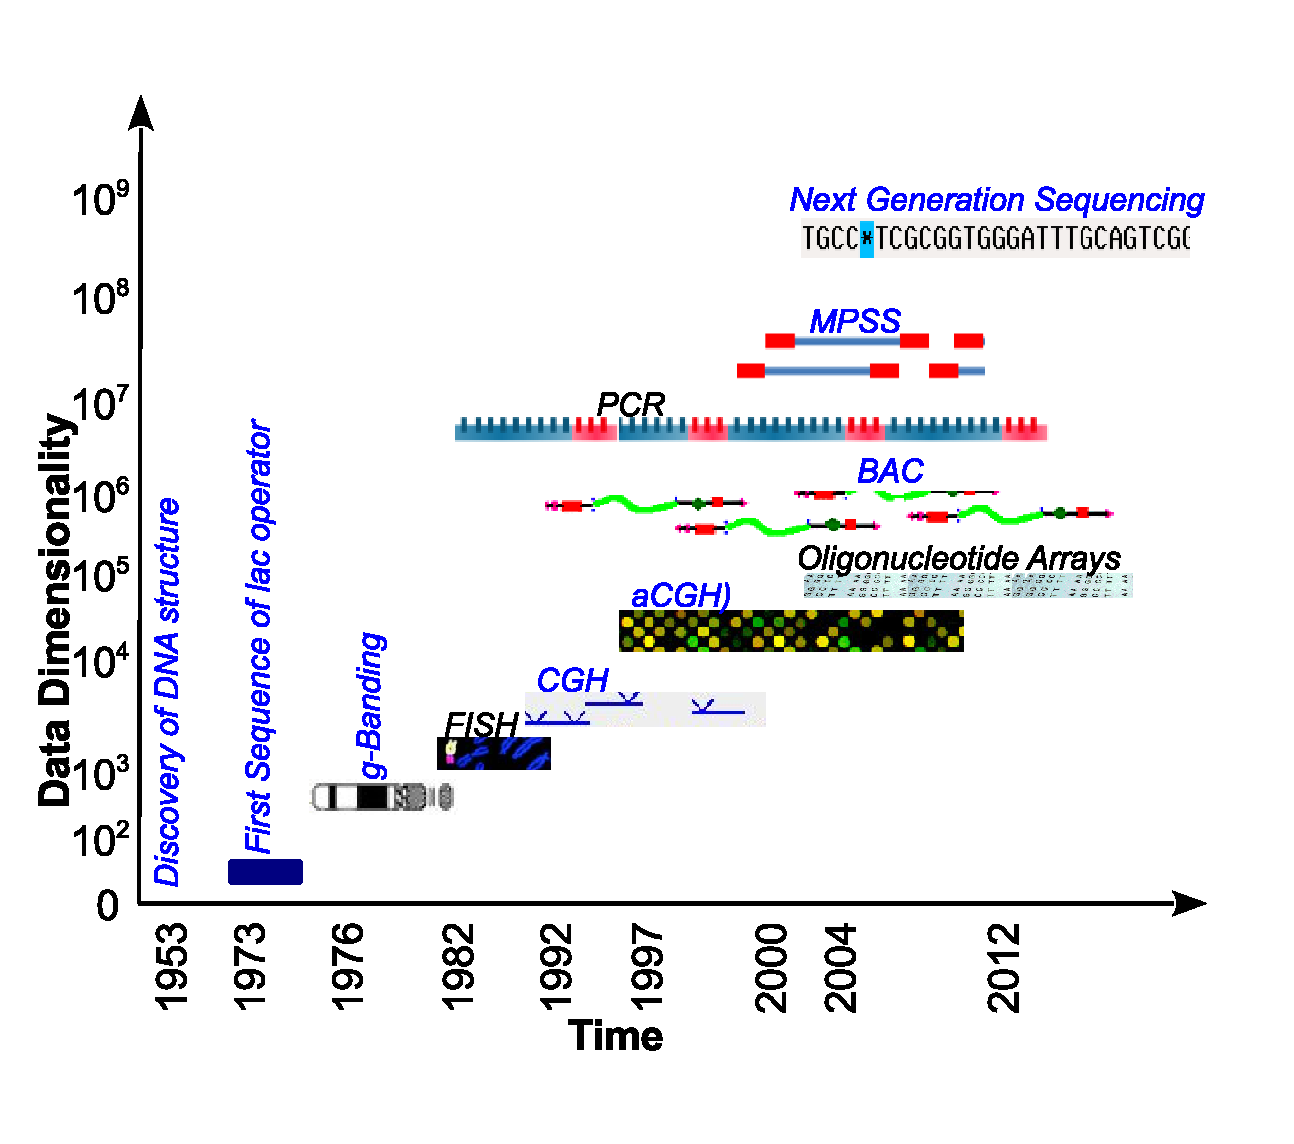
\includegraphics[trim=10mm 20mm 20mm 2mm,width=0.99\textwidth]{figures/arraytypes}
\caption[Evolution of measurement in biology.] {Evolution of measurement technology
in biology described in terms of their level of detail in measurements and time of usage. } 
\label{Fig:arraytypes}
\end{figure}

Years of evolution and adaptation have made organisms complex biological 
beings~\cite{mcshea1991}. Ever improving measurement technologies have also 
provided the facilities to measure the complex phenomena in biology~\cite{united2009new}. 
After the discovery of DNA in 1953~\cite{watson1953dna}, different measurement
methods have been proposed to measure the ge\-nome. First sequence of lac 
operator of 
24 bp was published twenty years after the discovery of DNA in 1973~\cite{gilbert1973nucleotide}. 
Figure~\ref{Fig:arraytypes} summarises the evolution of DNA sequencing
technology from the 1973. Initially, different banding methods such as 
G--banding and Q--banding technologies were developed to produce a visible 
karyotype by staining the chromosomes~\cite{benn1992}. A karyotype here 
denotes the  set of all chromosomes in an organism. Alongside the banding 
technology, FISH (Fluorescence In Situ Hybridisation) was developed to
detect the presence or absence of DNA sequences on chromosomes. Similarly, 
microarray technologies such as the  Comparative Genomic Hybridisation 
(CGH)~\cite{kallioniemi92} and array Comparative Genomic Hybridisation 
(aCGH)~\cite{pinkel98} were developed to study the Copy Number Variations 
(CNV) without requiring culturing of cells. Additionally, Bacterial 
Artificial Chromosome (BAC) was developed to sequence the genomes of 
organisms. 


Similarly, Oligonucleotide arrays that uses oligos of short lengths 
(less than 25 bases) were developed to test large number of oligos 
in presence of smaller number of targets~\cite{lockhart96}. In 
addition, promoter arrays were developed to probe thousands of 
promoter sequences in one array experiment~\cite{wang2005}. 
Besides, Massive Parallel Signature Sequencing (MPSS) was developed
to analyse the level of gene expression by identifying and quantifying 
Messenger Ribonucleic Acid (mRNA) transcripts in the sample~\cite{brenner2000mpss}. 
Likewise, Polymerase Chain Reaction (PCR) were developed to amplify
one or small number of copies of DNA thereby generating large number 
of copies of particular DNA sequences useful for biomedical application
such as DNA sequencing and diagnostic purposes~\cite{pcr2003}.

Around the beginning of this century new technology known as next 
generation sequencing (NGS) had resounding impact in DNA sequencing. 
In~\cite{mardis08} and~\cite{mardis2011}, authors summarise 
the improvement in DNA sequencing which has positive impact on the 
biomedical research providing high throughput and high resolution 
techniques to explore, and answer genomewide biological questions. 
%We have only shown two next generation sequencers in the Figure~\ref{Fig:arraytypes}. 
%Nevertheless, different vendors have produced different sequencers
%for commercial use~\cite{liu2012}.
The Carlson curve accurately predicted the doubling time of DNA sequencing 
technologies measured in terms of cost and performance~\cite{carlson2003}.
Furthermore, the curve illustrates the dramatic decrease in cost which is 
sometimes hyperexponential and similar dramatic improvements in technology
to measure biological phenomenon such as DNA sequencing and synthesis, 
gene expressions, and protein structures.

These improvement in measurement technology in biology over the 
period of time produces data in different representation. 
Consequently, multiresolution data are also present 
in biology. For example, measurements from an older generation
technology (eg. G--banding) can be represented in data with
dimensionality in hundreds~\cite{benn1992,shaffer05}. 
In contrast, newer generation technology such as 
microarray measures the same karyotype generating the
data of dimensionality of thousands~\cite{kallioniemi92,pinkel98}. 
In addition, latest technology known as Next Generation Sequencing 
produces the data with millions of dimensions~\cite{mardis08,roh10com}.

The Figure~\ref{Fig:arraytypes} shows major changes in
sequencing technology. However, within each generation of technology
there are several minor improvements.  For example, aCGH 
improves the mapping resolution of 20Mbp (Megabase Pairs) to 100 
Kbp (Kilobase Pairs) over its predecessor CGH.
Similar methods within a generation of technology  also produce
data in different resolutions because  of improvements within 
the technology such as microarrays and banding. For example, authors 
in~\cite{usvasalo2010} use microarray data in two resolutions of 
44000 and 244000 measurements per microarray measured by Agilent 
44B and 244A aCGH platforms to classify different types of leukemias.
Similarly, in NGS, different vendors have produced different sequencers
for commercial use~\cite{liu2012}.

Studying the data generated by different technologies above produces 
wide range of benefits, especially in understanding of the biological
phenomenon. Therefore, computational methods have been used 
to analyse the generated data. The phenomenon of doubling of 
number of transistors in a chip within 18 to 24 months, often known as 
Moore's Law~\cite{moore1965}, has improved the processing power of 
computers exponentially. Similarly, with the advent of Internet and 
other communication technologies and protocols; communication systems
have also improved dramatically. The data storage capacity is also
rapidly rising. These  advancements have resulted in  improved 
computing power thus facilitating development of novel algorithms
to analyse the generated data.

\subsection*{Pan--cancer Analysis}
\label{ss:pancancer}

In addition to the data in different resolutions, efforts have 
been made to study different cancer types by collecting data from 
different sources in pan--cancer  initiative~\cite{pancancer}. 
The aim of the study is to develop an integrated picture of
commonalities, differences, and emergent themes across tumour 
lineages. The initiative involves multiple datasets and 
multiple cancers showing possible utility of multiresolution methods 
in pan--cancer initiative. In the previous
research of our research group, we have considered all cancers 
within a single analysis~\cite{myllykangas06}.



\section{Multiresolution Chromosomal Amplification Data}
\label{s:multchrdata}

Similar to the array technology and next generation sequencing, 
the International System for human Cytogenetic Nomenclature (ISCN)
has defined five different resolutions of the chromosome namely:
300, 400, 550, 700, and 850 in G--banding~\cite{shaffer05}. Each resolution 
defines the precision in division of karyotype. 
For example, in coarse resolution, a karyotype is divided into 
312 ($\approx 300$) different regions, i.e., with lower precision.
In contrast, in fine resolution, a karyotype is divided into 862
($\approx 850$) different regions, i.e., with higher precision
compared to resolution 300.


%%%%%%%%%%%%%%%%%%%%%%%%%%%%%%%%%%%%%%%%%%%%%%%%%%%%%%%%%%%%%%
%%%%%%%%%%%%%%%% chromosome 21 figure drawn goes here %%%%%%%%


\begin{figure}[h!]
\centering
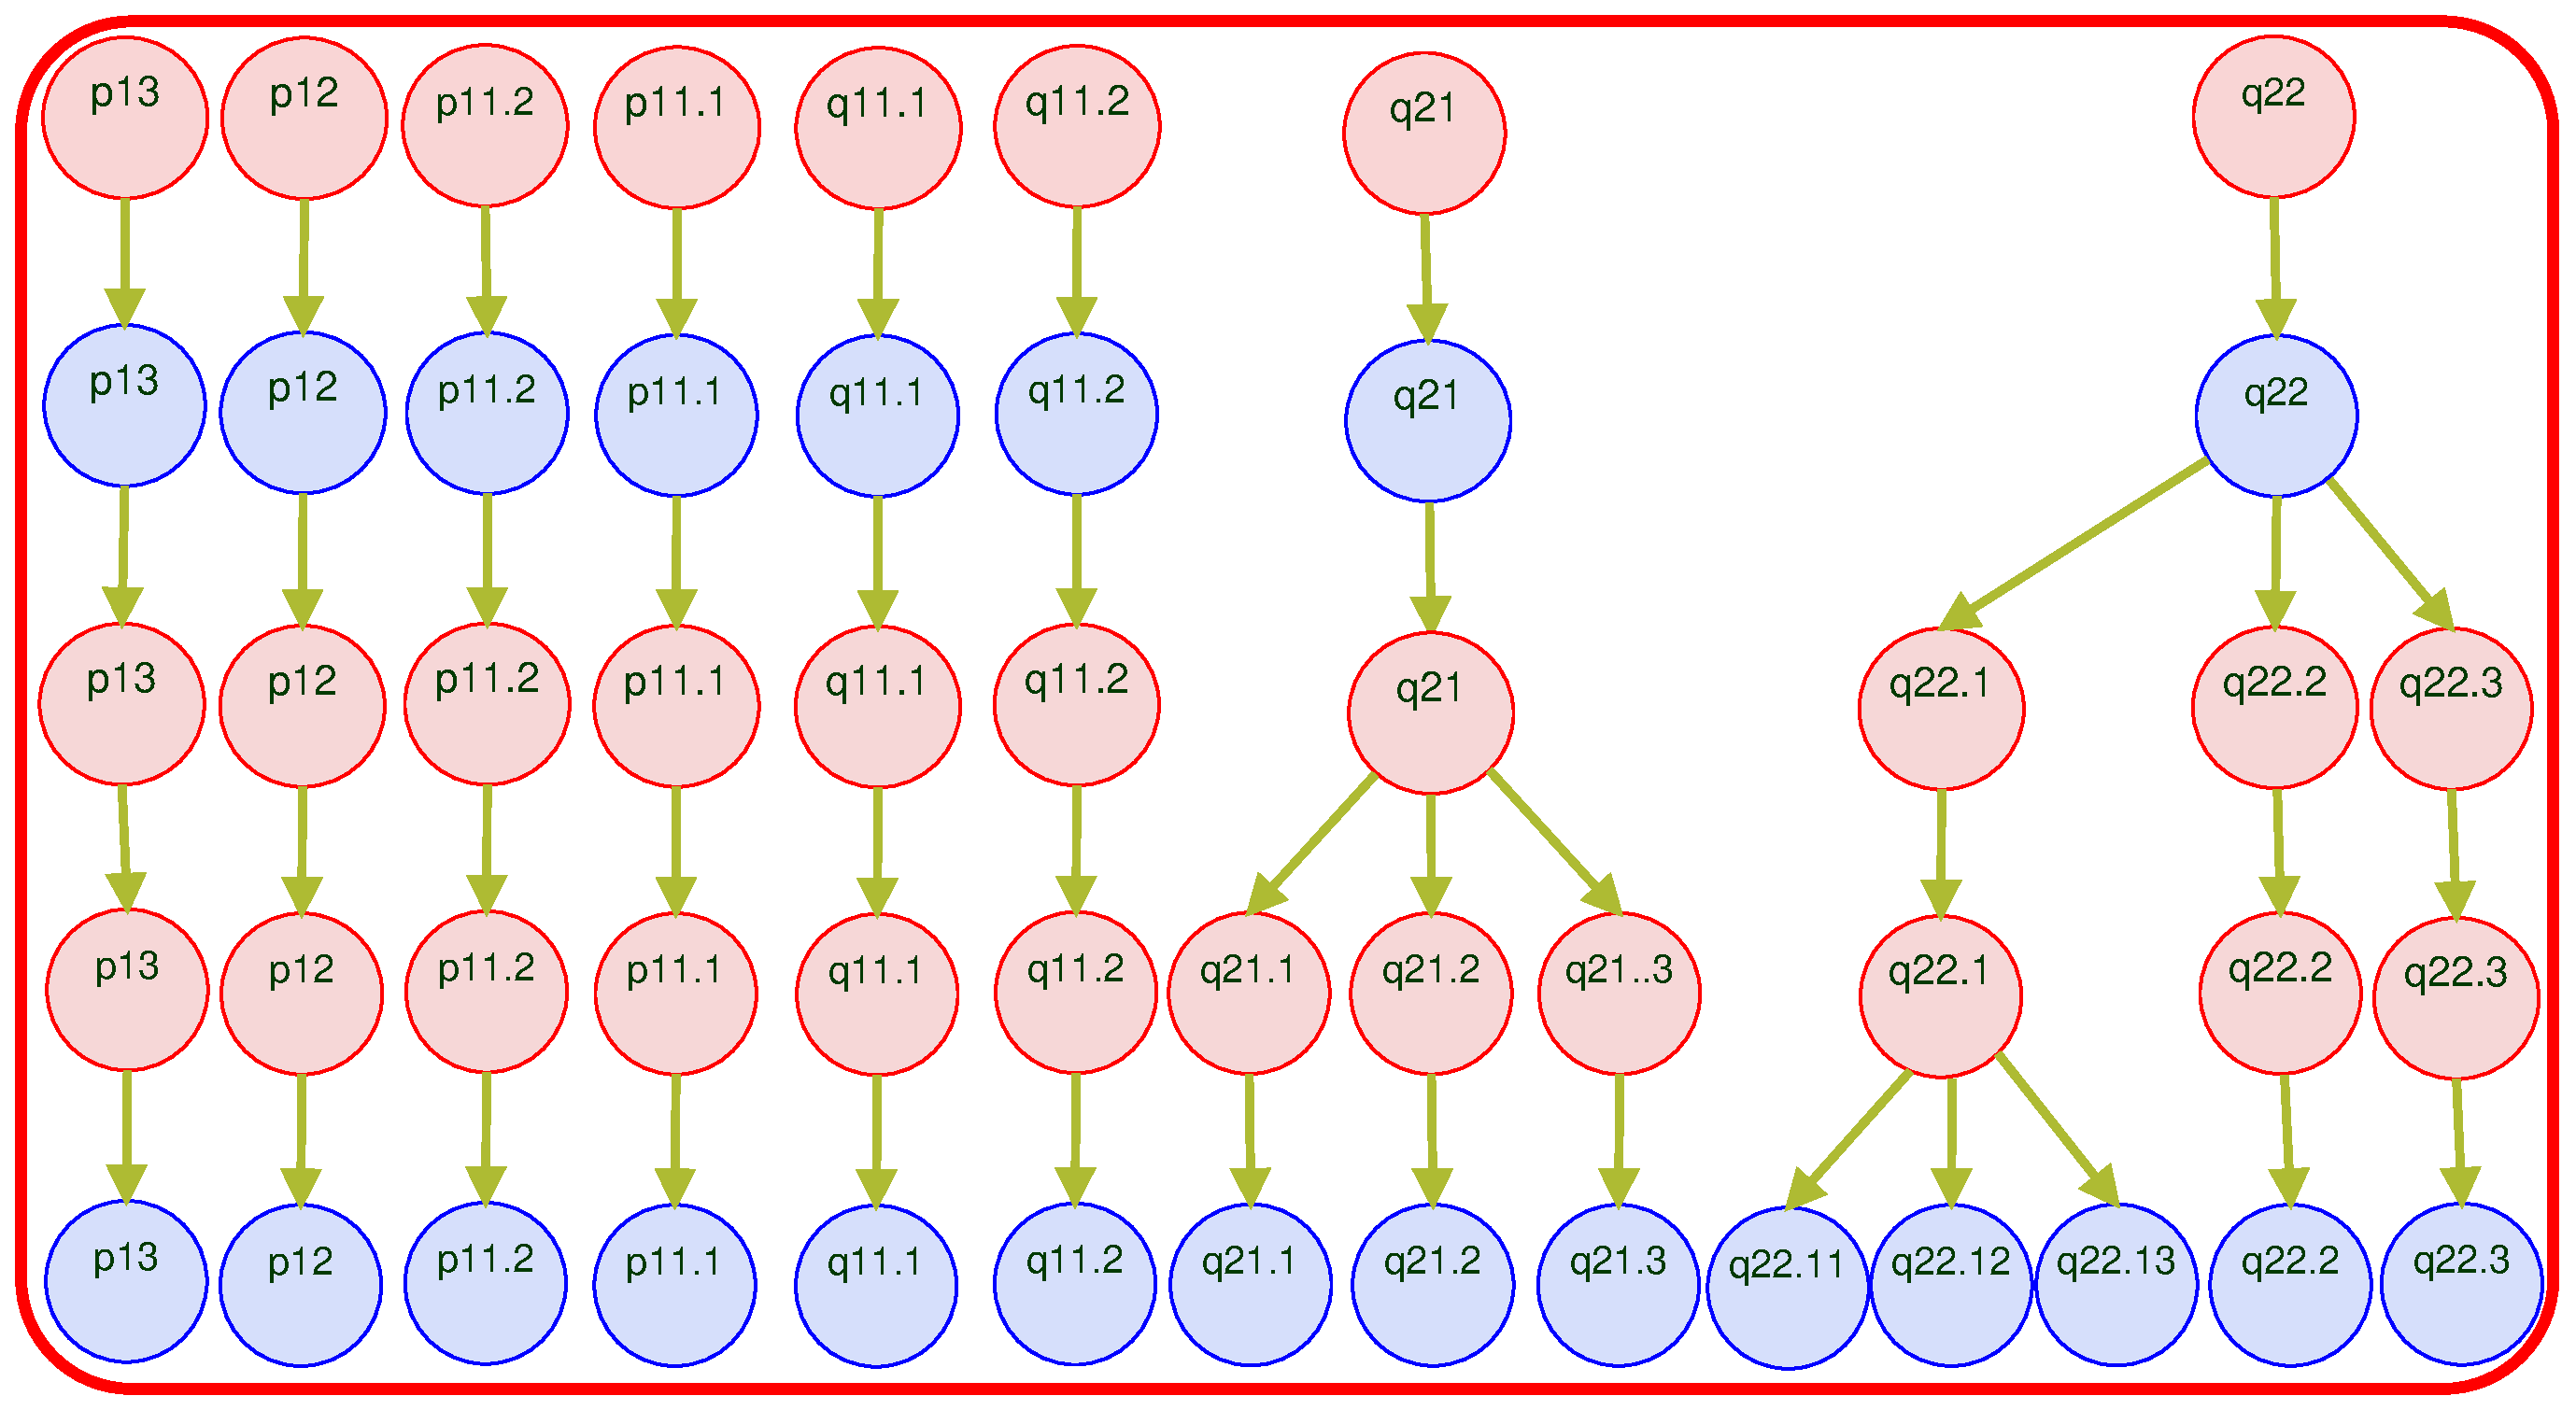
\includegraphics[trim=10mm 5mm 20mm 0mm,width=0.99\textwidth]{figures/chain}
\caption[Multiple Resolutions of the Genome.]{A typical 
relationship between multiple resolutions of genome.  
Figure shows chromosome 21 in five different resolutions 
of genome as defined by ISCN standard. The division is irregular,
and hierarchical but consistent because of the ISCN standard.
Chromosome 21 is chosen for the clarity of the presentation 
because it is the smallest chromosome. Y--axis denotes different resolutions
of genome while x--axis denotes spatial coordinates (different regions) of the genome.
Figure is adapted from~\citepub{c3}.} 
\label{Fig:chr21}
\end{figure}


%%%%%%%%%%%%%%%%%%%%%%%%%%%%%%%%%%%%%%%%%%%%%%%%%%%%%%%%%%%%%%

Figure~\ref{Fig:chr21} shows five different resolutions in 
chromosome 21 according to the ISCN standard. The figure depicts 
the division of regions and chromosome nomenclature with 
an example in chromosome 21. Chromosome 21 is chosen 
for visualisation because it is the smallest chromosome. Chromosome 21 is
divided into 8, 8, 10, 12, and 14 regions in resolution
300, 400, 550, 700, and 850. The nomenclature of the regions 
and their division in different resolutions are irregular 
and hierarchical~\cite{shaffer05}. Some regions are  
undivided whereas other regions are divided into  
different number of regions. For example, the regions 21p12 and 
21p13 are undivided in all the resolutions where as the 
region 21q22 is  divided into 3 and 5 different regions 
in resolution  550 and 850. This division of karyotype
in different levels of detail allows 
measurement technologies to generate data in multiple
resolutions. Each chromosomal region in coarse 
resolution is related with a chromosomal region in
fine resolution with a one to many relationship. 
Given the measurements of same subject in two different
resolutions, the aberrations should be consistent with
each other, i.e., the aberrations should be the same except for some 
measurement errors.

%%%%%%%%%%%%%%%%%%%%%%%%%%%%%%%%%%%%%%%%%%%%%%%%%%%%%%%%%

%data21multi
\begin{figure}[h!]
\centering
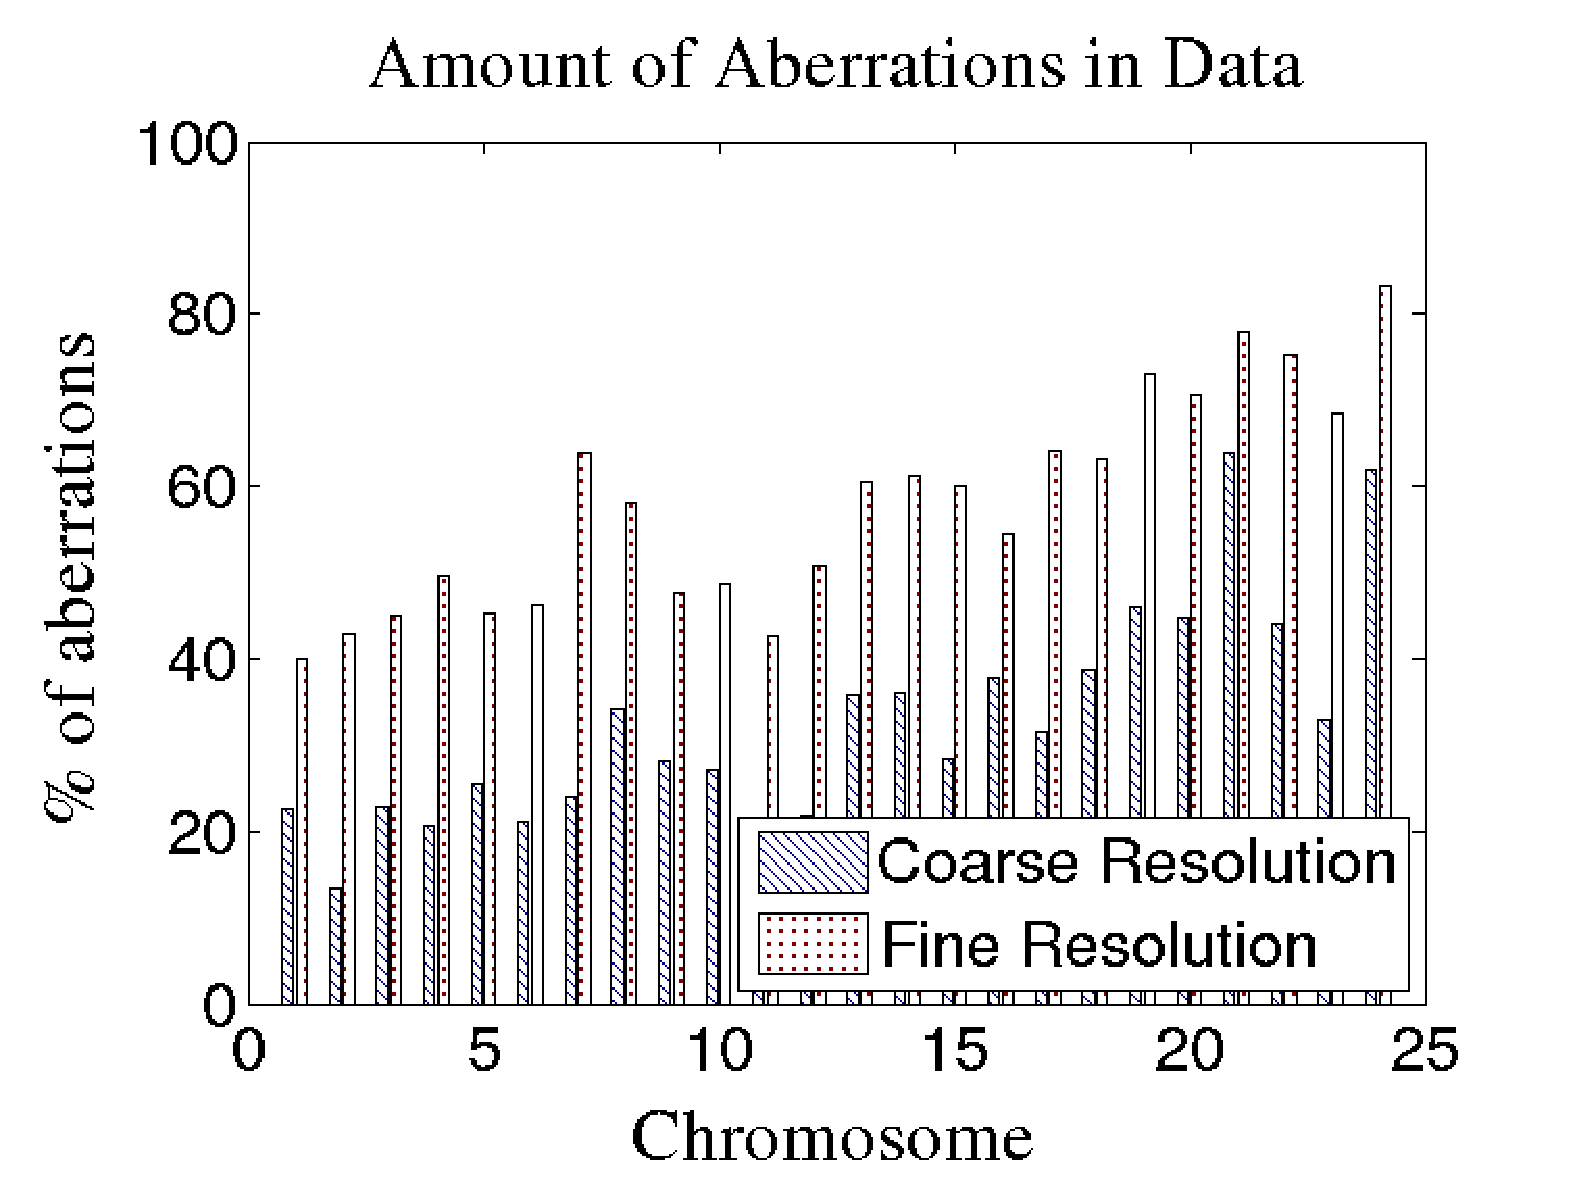
\includegraphics[trim=5mm 2mm 18mm 2mm,width=0.99\textwidth]{figures/perabar}
\caption[Amount of Aberrations in Different Chromosomes]
{Amount of aberrations in each chromosome in two datasets in different data
resolutions. The bar diagram shows that chromosomes in fine resolution 
are comparatively more aberrated than the coarse resolution.} 
\label{Fig:perabar}
\end{figure}


%%%%%%%%%%%%%%%%%%%%%%%%%%%%%%%%%%%%%%%%%%%%%%%%%%%%%%%%%%%%%%%%%%%%%%%%%%%%%

For the experiments, two different datasets were available
in coarse resolution and fine resolution. Researchers at 
the University of Helsinki compiled a dataset of chromosomal 
amplification in coarse resolution reading through the 
literature published between 1992--2002~\cite{knuutila2000}. 
All 838 journal articles were read through manually.
The data describes the chromosomal amplification patterns of 
4590 cancer patients in coarse resolution, i.e., resolution 
400 where a karyotype is divided into 393 different regions.
Similarly, data in fine resolution extracted 
from~\cite{progenetix,baudis07} describes chromosomal
amplification in fine resolution, i.e., resolution 850 where
a karyotype is divided into 862 different regions. Since the 
cancer patients were not the same, there is no direct 
correspondence between data samples in two different 
resolutions. Therefore, most of the analysis methods 
discussed in this thesis consider unsupervised methods
which learn the hidden structure in the data without the 
help of the class labels~\cite{bishop06,mitchell97}.
If the measurements were available from the same cancer patients
in two different resolutions, we can expect consistent matching 
in aberrations except for measurement errors.

In the coarse resolution data, a total of 26527 (out of 1,803,870) matrix elements
are aberrated which accounts for approximately 1.5\% of the total matrix 
elements in the dataset. In all our experiments, we  process 
the data chromosomewise to reduce the data dimensionality and 
with the expectation of finding chromosome specific patterns 
to describe different cancers. When the data is divided into 
each chromosome, there are some samples which do not show 
aberration in any of the chromosomal regions. Such data samples
are deleted as we are interested in modelling chromosomal aberration
patterns and their relation to cancer, not their absence.
Therefore, number of samples and data dimensionality
in each chromosome is different. We therefore calculate percentage
of aberrations in each chromosome in each resolution for comparison purposes. Figure~\ref{Fig:perabar} 
depicts the amount of aberrations in both coarse resolution 
and fine resolution data. Data in fine resolution shows more 
aberration than the data in the coarse resolution. The percentage 
of aberrations are approximately 50\% overall, while the minimum 
and maximum are approximately 15\% and 80\% respectively.



\begin{figure}[h!]
\centering
\includegraphics[trim=10mm 10mm 20mm 2mm,width=0.99\textwidth]{figures/data21multi}
\caption[Multiple Resolution in Chromosome 21.]
{Visualisations of data describing chromosome 21 in two different 
resolutions: 300, and 850. Each sample, i.e., each row denotes one 
cancer patient and each column determines a chromosomal region. 
The black colour denotes presence of amplification and white col or 
denotes the absence of amplification. The two different panels in 
the figure depict the same phenomenon measured at different resolutions.
Some chromosomal regions (variables or features in machine learning 
terms) such as 21p21 in left panel have been divided into different 
regions such as 21p21.1, 21p21.2, and 21p21.3 in the right panel. 
Figure is adapted from~\citepub{j1}.} 
\label{Fig:datamulti}
\end{figure}

%%%%%%%%%%%%%%%%%%%%%%%%%%%%%%%%%%%%%%%%%%%%%%%%%%%%%%%%%%%%%%%%%%%%%%%%%%%%%

Figure~\ref{Fig:datamulti} depicts five samples of data from 
chromosome 21 in both the coarse and the fine resolution.
In the Figure~\ref{Fig:datamulti}, rows denote the cancer patients 
and the spatial coordinates on the X--axis denote the chromosomal 
region.  In addition, white colour denotes value of zero (0), i.e.,
the absence of amplification, and  black colour denotes the value 
of one (1), i.e., amplification in that specific region of genome 
for that specific cancer patient. The left panel of the  
Figure~\ref{Fig:datamulti} shows that one region 21p21 in coarse 
resolution is divided into 3 regions in the fine resolution:  
21p21.1, 21p21.2, and 21p21.3 as shown in the right panel of the
figure. In contrast, some of the regions such as 21p13 and 21p12 
are same in both coarse and fine resolution. 
%Therefore, different regions are divided differently. 
Some regions are undivided while other
regions are divided into varying number of regions. Nevertheless, 
the division is consistent because of the ISCN standard. Detailed 
description of the amplification dataset in coarse resolution 
can be found  in~\cite{myllykangas06}.








%%%%%%%%%%%%%%%%%%%%%%%%%%%%%%%%%%%%%%%%%%%%%%%%%%%%%%%%

\section{Ontology of Multiresolution Data}
\label{s:ontologymulti}

The concept of ontology transcends back to the dates of noble 
philosophers Aristotle, Parmenides, and Jacob Lorhard, who 
used the term ontology in the philosophical context to
describe the state of being, and reality~\cite{cohen2014}.
Recently, the term ontology has found its prominence 
in computer and information science community. 
In computer science community, ontology is 
the mechanism for explicit description of the 
conceptualisation of the knowledge represented in the 
knowledge base~\cite{gruber1993,swartout1996}. 

Ontology is a popular methodology to describe the semantics of the 
data in machine learning and data mining community~\cite{panov2012}. 
Recent studies have shown that relevant additional knowledge enhances 
the knowledge discovery process of empirical data~\cite{panov2012}. 
Expansion of semantic web and increasing 
availability of domain knowledge as  ontologies has resulted
in  growth of semantic data. Semantic data mining algorithms
address the challenge of mining abundance of knowledge 
encoded in domain ontologies constrained by the heuristics 
computed from the empirical data~\cite{Vavpetic13jiis}. 

Multiresolution data conceptualises one of the essential 
ontological dichotomies of universals and particulars
in metaphysics~\cite{so49866,russell1911}. The data
in the coarse resolution can be conceptualised as 
universals whereas data in fine resolution can be 
conceptualised as particulars. Therefore, we 
can use ontological information in modelling 
multiresolution data as in~\citepub{c3} and \citepub{j2}.

Biological systems are complex consisting of many interwoven subsystems that 
effect the functionalities of each other~\cite{kim2003}. As a result, 
chromosomal amplifications can effect, and be effected by other 
biological phenomenon. Furthermore, cancer is a multifactorial 
disease and the heterogeneity of cancer also suggests that biological 
phenomenon besides chromosomal aberration can catalyse the development
of cancer. For this reason, additional background knowledge in biology 
was used to enhance the comprehensive analysis of chromosomal 
amplification datasets and to help understand the phenomenon of cancer. 
The additional knowledge used in the analysis of multiresolution data 
are the taxonomy of hierarchy of chromosomal regions, the cancer genes,  virus 
integration sites, fragile sites, and ampli\-fication hotspots
in~\citepub{j2}. Only taxonomy of hierarchy of regions is used
as background ontology in~\citepub{c3}.

The mutations in genes resulting to a larger extent by ``acquired 
mutation'' and to a lesser extent by ``germline mutation'', known 
as cancer genes, are one of the most prominent causes of 
cancer~\cite{futreal2004}. Authors in~\cite{futreal2004} have 
listed the cancer genes and compared them to the complete gene
set revealed by the human genome sequence. Similarly, fragile 
sites are nonrandomly distributed loci on human  chromosome 
that show a constriction or a gap and increased frequency of 
chromosome breakage under the conditions of partial 
replication stress~\cite{durkin07,schwartz06}. The fragile 
sites are often found rearranged in cancers~\cite{glover2005}. 
Virus integration sites are the locations in chromosome where 
the viral Deoxyribonucleic acid (DNA) inserts into host cell 
DNA~\cite{khoury2013}. Viruses are responsible for approximately 
12\% of cancers~\cite{khoury2013,zurHausen2009}. Amplification 
hotspots are frequently amplified chromosomal locations in cancer 
patients identified using computational modelling in~\cite{myllykangas06}.
The semantic data mining methods use these additional knowledge  
to enhance the knowledge discovery process in~\citepub{j2} in 
semantic subgroup discovery framework.

\section{Pattern Mining}
\label{s:patternmining}

Pattern mining is a popular branch of data mining that aims to 
extract interesting, relevant, and meaningful patterns from the 
data~\cite{han2007,hand01}. Frequent itemset mining 
is one of the first and most popular pattern mining algorithm. 
Itemsets are a set of items or columns in a 0--1 
dataset having high concentration of 1s and are used as 
patterns in a 0--1 dataset~\cite{tatti08}. 
Let $\mathcal{I}_1,\mathcal{I}_2,\ldots,\mathcal{I}_n $ be the 
attributes (items) of a dataset, $\mathcal{D}$, and $\sigma$ be 
the given support. A frequent itemset is 
a set $\mathcal{F}$ of items of $\mathcal{D}$ such 
that at least a fraction of $\sigma$ of the rows of $\mathcal{D}$ 
have 1 in all columns of $\mathcal{F}$~\cite{agrawal1993,mannila1994}.

Anti--monotone property of frequent itemset suggests that if an 
itemset is frequent, then all its subsets %$\lbrace a,b,c \rbrace$
are also frequent~\cite{gallo2008}. Hence frequent itemsets 
generate a larger number of patterns making it difficult to 
report and interpret the results. Maximal frequent itemset 
ameliorates challenges posed by larger number of patterns
in frequent itemsets. An itemset is maximal frequent if none 
of its immediate supersets is  frequent~\cite{burdick01}. 
We use maximal frequent itemset  in~\citepub{c1} to compare 
and report patterns across different resolutions.

Similarly, association rule is a popular data mining methodology 
to determine the interesting relations between variables based 
on different measures of 
interestingness~\cite{agrawal94,hipp00,klemettinen94,piatetsky91b}. 
Most initial studies in association rule mining focused 
on finding interesting patterns from the large databases
in an unsupervised setting. Nevertheless, association rules have 
been used in classification~\cite{jovanoski01,liu98}. 
Continuing with the research on association rules and classification, 
domain of subgroup discovery has emerged as a popular data mining 
methodology for labelled data. Subgroup discovery aims at finding 
interesting rules from the data that  best describe the target 
variable~\cite{gamberger02,franciso11,novak09}. Additionally, 
contrast set mining aims to learn the variables that 
differentiates one group of target variables from the rest, i.e., 
the most discriminating sets of variables~\cite{bay01,novak09}.


Semantic data mining method is a branch 
of data mining that uses taxonomies and ontologies of background data 
to improve the performance of 
algorithms~\cite{lavrac2011,AnzeCJ2012,Vavpetic13jiis}. 
Semantic data mining has recently gained research 
interest in pattern mining community because of the availability 
of large amount of data in the form ontologies encoded in semantic
web~\cite{lavrac2011}.  Especially, the additional knowledge are 
abundantly available in biology as discussed in 
Section~\ref{s:ontologymulti}. In~\citepub{j2},
we use semantic data mining algorithm to explain the clustering 
results obtained by probabilistic clustering using background knowledge
discussed in Section~\ref{s:ontologymulti}.

\section{Related Work in Multiresolution Data Analysis}
\label{s:relatedMultiRes}

Multiresolution analysis and modelling research community is growing steadily because 
of the pragmatic approach in dealing with datasets in different 
representation within a single analysis and also because of the 
increasing availability of multiresolution data in different 
application areas~\cite{barth2002multiscale,he2000wavelet,iske2004}. 
For instance, authors in~\cite{reddy2007} have % used multiresolution strategy to 
improved the efficiency of boosting algorithms in regression and 
classification, using the model--driven and data--driven multiresolution
strategy. Similarly, multi\-resolu\-tion trees have been used for object
recognition in homogeneous data based on recursive neural 
networks~\cite{bianchini2006}. In addition,
multiresolution visualisations have been used to visualise  
large volumes of complex data using semantic analysis to 
infer increasing levels of meaning from the data~\cite{hussain11}.
Similarly, tree structured self--organising maps (TS--SOM) have been 
proposed in the literature as a multiresolution representation of
several self--organising maps (SOMs)~\cite{koikkalainen94}.


\subsection*{Multiresolution Probabilistic Models}
\label{s:multiresProMdl}

Multiresolution modelling has also received research interest in 
probabilistic modelling domain. Most of the focus in this thesis
has been the use of probabilistic models, namely mixture models,
to analyse multiresolution  data. Traditional machine learning 
and data mining methods, such as mixture models, are unable to 
analyse  multiresolution data in their standard form because  
of the difference in representations of data in different  
resolutions.
%Likewise, 
%mixture models are also unable to model multi\-resolution data in 
%their standard form. 
The only approach to model multiresolution data is 
to model each resolution separately and at best compare the results.
Nevertheless, multiresolution models have found their usage in the 
literature, especially, in the image processing domain. 
For example, multi\-resolution kd--trees have been used to improve the performance 
of mixture models and reduce the cost associated with the Expectation 
Maximisation (EM) algorithm~\cite{moore99veryfast}. Similarly,
multiresolution kd--trees have also been used to build robust models
against the outliers using the EM algorithm~\cite{ng03robust}. 
Similarly, multiresolution binary trees have been used to store
probability values  efficiently both in terms of time and memory~\cite{bellot2003}.

Authors in~\cite{mukherjee13} have improved
the performance of Gaussian Mixture Model (GMM) using wavelet subbands
with an additional feature of incorporating variable number of
components in the GMM. The GMM in~\cite{mukherjee13} can use any 
multiresolution based decomposition for background suppression.
Authors in~\cite{wilson00} show that Multiresolution Gaussian Mixture 
Model (MGMM) adapts to smooth motions. The authors then apply the MGMM to 
estimate the visual motion. Similarly, authors in~\cite{meila2000} 
propose efficient algorithms to learn a mixture of trees model in 
a maximum likelihood and Bayesian network framework for discrete 
multidimensional domains. 


\subsection*{Related Areas}
\label{s:relatedAreas}

Multiresolution analysis and modelling shares commonality with 
various research areas and applications. The following sections
briefly review the work on multiresolution modelling in the 
relevant research areas.

\subsubsection{Multiscale Analysis and Scale space Theory}
\label{ss:scalespace}

Multiresolution modelling is often synonymously used in 
literature with the scale space theory~\cite{Lindeberg94b} 
and also multiscale analysis~\cite{e2011principles}. 
In image processing domain, pyramid structures generated 
after successive smoothing, and subsampling produces a 
multiscale representation~\cite{Lindeberg94b}. Similarly, 
in scale space theory a scale parameter, $t$, handles 
images at different scales. Scale space representation, 
an improvement over multiscale representation, has an 
ability to compute representation at a desired scale. 
Authors in~\cite{babaei2013} address an important challenge
in cancer research by identifying densely connected 
components of known and putatively novel cancer genes
in protein protein interaction networks using a 
multiscale diffusion kernel. The results in~\cite{babaei2013}
demonstrate the importance of multiscale analysis as
the putative cancer genes and network are significant 
at different diffusion scales. Similarly, authors 
in~\cite{ridder07} detect statistically significant co--mutations
in multiple independent insertional mutagenesis screens. The 
significance is estimated on multiple scales and results are visualised
in  scale space thus providing valuable supplementary information 
on the putative cooperation.
Multiscale analysis and scale space theory
also provide functionalities to address
the challenges of image representation at different resolutions. 
Similarly, a family of methods known 
as super--resolution has been used to increase the resolution 
of images and videos~\cite{milanfar2010super}.
Generally, both 
multiscale and scale space methods work in model 
domain. 
%This is also because the smoothing parameter, 
%$t$, in scale space method smooths out the 
%image structures smaller than the size, $\sqrt{t}$.
However, multiresolution methods developed in this thesis
are the result of multiresolution challenges arising in 
the data domain. 


\subsubsection{Wavelets}
\label{ss:wavelets}

Wavelets are appropriate methods to describe the mathematical 
phe\-nom\-e\-non such as functions and signals at different levels 
of resolution~\cite{mallat89}. Wavelet analysis have been 
popular tool in multiresolution analysis~\cite{jawerth94}.
However, the classical wavelets based techniques are useful 
in regular, consistent, and  homogeneous setting. Hence, 
wavelets cannot directly handle the irregularities in the 
chromosomal amplification data.
%discussed in Section~\ref{s:multchrdata}.


\subsubsection{Learning from Multiple Sources}
\label{ss:lfms}

%Multiresolution modelling domain has a close affinity with the 
%domain of learning from multiple sources~\cite{crammer08}. 
%Improvement in measurement technology also increases the 
%dimensionality of the data. In practical applications, the 
%sample size of data is small, i.e., ($N \ll d$), where $N$ 
%represents the number of data samples and $d$ represents 
%data dimensionality. 
Similar to multi\-resolution modelling, 
learning from multiple sources aims to ameliorate the 
problem of curse of dimensionality, or Hughes effect by 
exploiting any related additional datasets 
such as earlier measurement experiments~\cite{crammer08}. 
Unlike multi\-resolution modelling, the additional datasets 
may only be weakly related to the analysed dataset. The 
para\-digm of learning from multiple sources is extended 
to the paradigms of multiview~\cite{sun13multiview}, 
multiway~\cite{huopaniemi10ismb}, and 
multitask learning~\cite{caruna97}.

\subsubsection{Data Fusion}
\label{ss:dataFusion}

The domain of data fusion shares a common ground with the domain of 
multiresolution modelling. Data fusion integrates  multiple data and 
knowledge depicting the same real world phenomenon in a single,
logical, precise, and useful knowl\-edge base~\cite{goodman97math}.
Data fusion techniques are often used to combine data from multiple 
sensors in such a way that the inference from the combined data is
better than that from individual sensors.
Data integration approaches have also been widely used in bioinformatics 
domain. For example, authors in~\cite{gopal2005} have proposed 
integrated database and software system that enables retrieval and 
visualisation of biological relationships across heterogeneous data 
sources. Similarly, authors in~\cite{kettunen2003b} combined data 
from complementary Deoxyribonucleic Acid (cDNA) arrays and  
tissue microarrays (TMA) to study the molecular changes in malignant
pleural mesothelioma (MM). The study shows that novel proteins 
associated with cell adhesion  are expressed either directly or 
as a regulatory mechanism in MM. The process of data fusion takes 
place at the different stages of analysis but it is a common 
practice to merge the data at the earliest stage of analysis 
in a single resolution. Data fusion techniques have 
also been used in multiresolution analysis, especially in 
remote sensing~\cite{carter1998analysis}.

\subsubsection{Granular Computing}
\label{ss:granular}

Granular computing (GrC) has roots in multi\-resolution 
modelling~\cite{bargiela2003granular}. GrC is a 
multidisciplinary field of study comprising of the\-ories, 
methodologies, and tools to analyse data using the 
granules in data~\cite{Yao02agranular}. 
Granular computing aims to divide data into 
different intrinsic resolutions to solve a problem which 
resembles with multi\-res\-o\-lu\-tion
modelling framework. 

%Different measurement methods have been proposed to measure ge\-nome.
%Banding technology such as Giemsa banding (G--banding)  
%produces a visible karyotype by staining the 
%chromosomes~\cite{benn1992}. 
%Similarly, microarray technology such 
%as the  Comparative Genomic Hybridization (CGH)~\cite{kallioniemi92} 
%and array Comparative Genomic Hybridization (aCGH)~\cite{pinkel98}
%facilitates the study of Copy Number Variations (CNV) without the 
%need for culturing cells. Additionally, Bacterial Artificial 
%Chromosome (BAC) are used to sequence the genomes of organisms. 
%Similarly, Oligonucleotide arrays uses oligos  of short lengths 
%(less than 25 bases)~\cite{lockhart96}. In addition, promoter array
%probes thousands of promoter sequences in one array 
%experiment~\cite{wang2005}. 
%The Next Generation Sequencing Methods
%provide high throughput and high resolution techniques to explore, 
%and answer genome-wide biological questions~\cite{mardis08}.


%Similarly, wavelets analysis have been popular tool in 
%multiresolution analysis~\cite{jawerth94}. 

%form, thereby sharing a common ground with 
%the domain of multi\-resolution modelling. 

%% Explanation of data
%who happen to be our  collaborators 
%Without the  use of fancy text mining techniques. 

%For example, 
%in bioinformatics, older generation technology such as the 
%banding measures a karyotype and produces data of 
%dimensionality of hundreds. In contrast, 
%relatively newer generation technology such as microarray 
%measures the same karyotype and generates the data of 
%dimensionality of thousands. Additionally, latest technology 
%known as Next Generation Sequencing produces the data with 
%millions of dimensions~\cite{roh10com}.

%Both the scale space representation and the multi\-scale analysis works 
%in the model 
%domain where models represent single resolution data at 
%different scales. %utilizing them to produce better results. 
%~\cite{lindeberg94b}

% In contrast, multi\-resolution modelling problem arises in the data domain 
% where the same data generating system is measured in varying levels of detail. 
% Most methods in machine learning and data mining literature are 
% designed to work with single resolution data. Since, the dimensionality
% of different data resolutions is different, the usual approach is
% to model each resolution separately. Scale space methods and wavelets
% usually use a multi\-resolution analysis setting for the datasets in the 
% same resolution. Furthermore, the multi\-resolution scenarios where 
% wavelets and scale space methods have their usage require regular, consistent, 
% and homogeneous division of regions such as the pyramid structure in image 
% processing domain~\cite{wilson00}.

%Older generation technology measures the coarser units of the 
%phenomenon and generates data in coarse resolution. In contrast,
%newer generation technology measures finer units of the phenomenon
%and generates data in coarse resolution.

%Such part of hierarchy form the multiresolution data.
%as shown in the Figure~\ref{Fig:oncology}.
%In addition to the data in multiple resolutions,

%Machine learning algorithms 
%%%%%%%%%%%%%%%%%%%%%%%%%%%%%%%%%%%%%%%%%%%%%%%%%%%%%%%%%%%%%%%%%
%%%%%%%%%%%%%%%%%%%%%%%%%%%%%%%%%%%%%%%%%%%%%%%%%%%%%%%%%%%%%%%%%
% \subsection{Related work in Model Selection in Mixture Models}
% \label{ss:relatedmxmdl}
% 
% A plethora of criteria and methods have been proposed in the literature
% to determine the optimal number of mixture components in a mixture 
% model~\cite{mclachlanfmm}. For example, authors in~\cite{celeux07},~\cite{Figueiredo2002}, 
% and~\cite{oliveira05} provide comprehensive 
% review of deterministic, and stochastic and re sampling criteria for 
% model selection. Deterministic criteria consists of criteria such as
% Akaike Information Criterion (AIC)~\cite{akaike1973}, Bayesian 
% Information Criterion (BIC)~\cite{schwarz78}, Minimum Description
% Length (MDL)~\cite{rissanen1978}, and integrated classification 
% likelihood (ICL)~\cite{biernacki2000}. Similarly,  stochastic 
% methods includes Markov Chain Monte Carlo (MCMC)~\cite{bensmail97},
% re sampling methods includes bootstrapped likelihood ratio 
% test~\cite{McLachlan1987}. Similarly, authors in~\cite{woo2006}
% propose robust approach against model misspecification leading 
% to a best-fitting mixture density based on minimum Hellinger 
% distances. Authors in~\cite{chen2008}~and~\cite{huang2013model}
% use penalized likelihood method for model selection in mixture
% model.
% 
% Data likelihood is often used as 
% the measure of the quality of mixture models~\cite{mixmodelcv}.
% A well trained mixture model with appropriate number of mixture
% component better estimates the underlying data distribution and 
% produces high likelihood values for the unseen data. Furthermore, 
% cross--validation have been popular model validation technique
% in the literature~\cite{geisser1974,monsteller1968,stone1974}.
% Hence, in this thesis we use cross--validated log--likelihood as 
% a criteria for model  selection.

%Most of these initial studies in 
%pattern mining focuses on finding interesting patterns such
%as frequent itemsets from the large databases in an 
%unsupervised setting. 

%Among these five 
%resolutions, resolution 300 divides the karyotype with lower 
%precision whereas resolution 850 divides the karyotype with
%higher precision.  
\chapter[Mixture Models and Model Selection]{Mixture Models and Model Selection}
\markboth{Mixture Models and Model Selection}{}
\label{ch:mixmodels}

\begin{fquote}[Samuel Karlin]The purpose of models is not to fit the data but to 
sharpen the questions.\fqsource{$11^{th}$ R A Fisher Memorial Lecture (1983)} 
\end{fquote} 

\begin{synopsis}
This chapter introduces mathematical foundation and 
formulation of mixture models. The chapter also discusses the
model selection in mixture models.
This chapter also discusses one of the associated publications
where we propose a computationally efficient algorithm to train
a series of mixture models to aid model selection procedure.
\end{synopsis}

Classical probability distributions such as Gaussian, Bernoulli, and 
Poison provide methods for probabilistic modelling 
of data~\cite{walpole2012}. However, in the real world scenario, 
a single probability distribution cannot emulate the complexity 
in the data. Nevertheless, a combination of sufficiently large number 
of probability distributions can possibly emulate complexity in the data. 
Such combination of multiple classical probability distributions 
forms a mixture model. Formally, mixture models are semiparametric 
latent variable models that model a complex data distribution by
weighted sum of different probability 
distributions~\cite{bishop06,everittmixdist,mclachlanfmm}. 

The probability distributions within a mixture model, known as 
component distributions, describe the observations present in the 
data. The formulation of mixture model involves determining the 
number of components in the mixture model, their associated 
distribution, and identification of the component
generating the specific data sample~\cite{mclachlanfmm}. 
Mixture models are often used  in hard clustering analysis as in 
this thesis. In hard clustering, only one component is responsible 
to generate a  specific data sample. Mixture models also provide 
the option of learning soft clustering.  In soft clustering, 
a data sample belongs to more than 
one cluster with a certain degree of association~\cite{bishop06}. 
A standard formulation of the mixture model assumes that the samples 
are independent and identically distributed (IID). Under the assumption 
that data originates from a known number of components, $J$, the 
probability density of a mixture model can be expressed as the weighted
sum of its component distributions as:

\begin{eqnarray}
\label{eq:mixmodel}
 p(x)=\displaystyle\sum_{j=1}^{\mathrm{J}} \pi_j P_j(x \mid \boldsymbol{\theta}_j),
\end{eqnarray}

where $j$ indexes the component distributions. In the 
Equation~(\ref{eq:mixmodel}), the mixing proportion 
(mixing or mixture coefficient) is denoted by $\pi_j$ for the $j^{th}$
component in the mixture model. It determines the weight of the 
component distribution in the overall mixture model. 
Mixing proportions satisfy  the property of convex combination such that 
$\int p(x)dx=1$, $\pi_j > 0$, and $\sum_{j=1}^{J}\pi_{j}=1$~\cite{everittmixdist}. 
Similarly, the parameters $\boldsymbol{\theta}_j$ in  
Equation~(\ref{eq:mixmodel}) denotes  the parameters 
of the $j^{th}$ component distribution of the mixture model.
Application area dictates the choice of distributions, which 
in literature is dominated by the distributions from exponential 
family such as Gaussian, and  Dirichlet~\cite{mclachlanfmm}. 
In this thesis, Bernoulli distribution is the preferred distribution 
because the datasets are 0--1 datasets describing chromosomal
amplifications.

\section{Mixture Models of 0--1 Data}
\label{s:mixmdl01}
Finite mixture model of multivariate Bernoulli distributions 
for a data\-set, $\boldsymbol{X}$, of
dimensionality, $d$, are parametrized by 
$\boldsymbol{\Theta}=\{J$, $\{ \pi_j,\Theta _j\}_{j=1}^{J}\}$. 
The data\-set, $\boldsymbol{X}$, consists of samples
$\mathbf{x}_1, \ldots, \mathbf{x}_N $ in such a way that
$\boldsymbol{X} = \{\mathbf{x}_1, \ldots, \mathbf{x}_N \}$.
Replacing the general probability distribution function with 
the distribution of choice, i.e., Bernoulli distribution, 
a mixture model of multivariate Bernoulli distribution can 
be mathematically expressed as~\cite{everittmixdist,wolfe70}:

\begin{eqnarray}
\label{eq:mixmdl01data}
p(\mathbf{x} \mid \boldsymbol{\Theta})= \displaystyle\sum_{j=1}^{\mathrm{J}} \pi_j \displaystyle \prod _{i=1} ^{\mathrm{d}} \theta_{ji}^{x_i} (1-\theta_{ji})^{1-x_i},
\end{eqnarray}

%As shown in the Equation~\ref{eq:mixmdl01data}, 
 
where $j$ indexes the components,
and $i$ indexes the data dimensionality. $x_i$ denotes the data point 
such that $x_i \in \lbrace 0,1 \rbrace$. The parameter of a random variable $\theta_{ji}$  
denotes the probability of the variable taking the value 1 in $i^{th}$ 
dimension of the $j^{th}$ component. We can collect all the random 
variables in a component in a vector, $\Theta _j$ such that
$\Theta _j=[\theta_{j1},\theta_{j2},\theta_{j3}, \ldots, \theta_{jd}]$.
Similarly, we can collect all the parameters of the mixture model including mixture
components in a matrix, $\boldsymbol{\Theta}$ such
that $\boldsymbol{\Theta}=\{J$, $\{ \pi_j,\Theta_j\}_{j=1}^{J}\}$.
The parameter values that maximise the log--likelihood function 
of the parameters can be defined using 
maximum likelihood principal~\cite{bishop06} as:

\begin{eqnarray}
  \label{eq:loglkhood}
  \mathcal{L} (\boldsymbol{\Theta} \mid \boldsymbol{X}) =\displaystyle\sum_{n=1}^{\mathrm{N}} \log  \left [ \displaystyle\sum_{j=1}^{\mathrm{J}} \pi_j \displaystyle \prod _{i=1} ^{\mathrm{d}} \theta_{ji}^{x_{ni}} (1-\theta_{ji})^{1-x_{ni}} \right].
\end{eqnarray} 
The EM algorithm can be used to learn the maximum likelihood parameters 
of mixture model of Bernoulli  distributions by maximising the likelihood 
in the Equation~(\ref{eq:loglkhood})~\cite{wolfe70}. 

\section{Expectation Maximisation Algorithm}
\label{s:emalgo}
Expectation Maximisation (EM) algorithm is an iterative algorithm
to determine the maximum likelihood (MLE) or maximum a posteriori 
(MAP) estimates of the parameters of latent variable 
models~\cite{expectmax,McLachlan2008emext}. The EM algorithm is a 
popular algorithm for learning model parameters in probabilistic 
latent variable models by maximising the marginal likelihood. 
The iterations of EM algorithm alternate between Expectation 
step (E--Step) and Maximisation Step (M--Step).

E--step estimates the posterior probability of each component 
for every data point. Whereas, M--step updates the  model parameters 
for next iteration. 
Iterations between E and M step produce a succession 
of monotonically increasing sequence of log--likelihood values
for the parameters $\tau\;=\;0,1,2,3,\ldots$ regardless of 
the starting point $\{\pi^{(0)},\Theta^{(0)}\}$~\cite{McLachlan2008emext}. 


\section{Model Selection in Mixture Models }
\label{s:mdlselectmix}

Model selection is the process of selecting a model of optimal complexity 
for the given set of (finite,training) data~\cite{cherkassky1998,hastie09}.
In the statistics literature, model selection is  the process of selecting 
a specific model from a plethora of choices~\cite{kadane04}. For example, 
in classification, model selection may refer to choosing a classification
algorithm from different classification algorithms such as Naive Bayes, 
Decision Trees, and Support Vector Machines. The focus in this thesis is 
modelling of a heterogeneous chromosomal amplification dataset.  
Mixture models are the model of choice because of their ability to model 
heterogeneity and their clustering capabilities. The choice of mixture
models is also motivated by their ability to learn the 
structure of the data better than most other methods because each 
component distributions capture dominant patterns in the data. Furthermore,
mixture models are scientifically proven as learning of mixture models 
involve well studied statistical inference techniques.

In this thesis, model 
selection refers to the model structure selection or complexity 
selection which determines the flexibility of the model to fit or 
explain the data. In other words, model selection in this context 
refers to choosing an appropriate level of model complexity in the 
selected class of model, i.e., mixture model. The complexity parameter 
in mixture  model is the number of component distributions in 
the mixture model. Model selection, therefore, is the selection 
of number of components in the mixture model~\cite{fraley1998}.

EM algorithm requires apriori knowledge of the number of components  
in the mixture model to learn the maximum likelihood parameters from
the data~\cite{McLachlan2008emext}. However, the number of component
distributions are often unknown apriori. Furthermore, one of the major
objectives of machine learning and data mining challanges in the real 
world can often be restricted to determining the number of components 
in the mixture model. Hence, model selection is essential to learn a 
mixture model using the EM algorithm.

A mixture model with large number of mixture components produces larger 
value for the log--likelihood in Equation~(\ref{eq:loglkhood}). However,
a mixture model with large number of mixture components also overfits 
the data, and generalises poorly on the future unseen data. Additionally, 
mixture models with large number of components increase complexity 
in training of mixture models with respect to both time and  memory.
In contrast, a mixture model with smaller number of mixture components 
underfits the data, and is unable to adequately represent 
the underlying data structure. Therefore, model selection aims to 
optimise this tradeoff between too simple and complex models.


\subsection*{Related work in Model Selection in Mixture Models}
\label{ss:relatedmxmdl}

A plethora of criteria and methods have been proposed in the literature
to determine the optimal number of mixture components in a mixture 
model~\cite{mclachlanfmm}. For example, authors 
in~\cite{celeux07},~\cite{Figueiredo2002}, and~\cite{oliveira05} 
provide comprehensive 
review of deterministic, stochastic and resampling criteria
for model selection. Deterministic criteria consists of 
Akaike Information Criterion (AIC)~\cite{akaike1973}, Bayesian 
Information Criterion (BIC)~\cite{schwarz78}, Minimum Description
Length (MDL)~\cite{rissanen1978}, and integrated classification 
likelihood (ICL)~\cite{biernacki2000}. Similarly,  stochastic 
methods includes Markov Chain Monte Carlo (MCMC)~\cite{bensmail97},
and resampling methods includes bootstrapped likelihood ratio 
test~\cite{McLachlan1987}. Similarly, authors in~\cite{woo2006}
propose a robust approach against model misspecification leading 
to a better fitting mixture density based on minimum Hellinger 
distances. In addition, the authors in~\cite{chen2008} 
and~\cite{huang2013model} use penalised likelihood method 
for model selection in mixture model.

Data likelihood is often used as 
the measure of the quality of mixture models~\cite{mixmodelcv}.
A well trained mixture model with appropriate number of mixture
components estimates the underlying data distribution better and 
produces high likelihood values for the unseen data. In addition, 
cross--validation have been popular model validation technique
in the literature~\cite{geisser1974,monsteller1968,stone1974}.
Hence, in this thesis we use cross--validated log--likelihood as 
a criteria for model  selection.


\section{Fast Progressive Training of Mixture Models}
\label{s:fast}

The EM algorithm is sensitive to initialisation and susceptible 
to local optima~\cite{McLachlan2008emext,wu1983}. One solution
to avoid local optima is to run the EM algorithm from different 
random initialisations and select the model with highest likelihood 
as the global optimum. Similarly, another solution is to take the 
average of different runs as general performance of the 
model~\cite{tikka2007b}. Furthermore, the  EM algorithm is 
computationally expensive because of its slow monotonic convergence 
property~\cite{McLachlan2008emext}. Therefore, multiple restart 
strategy is popular method in literature where the EM algorithm 
is run only for a small number of steps, i.e., not until 
convergence, generating large number of models. Among those models, 
the model with maximum likelihood can be selected
to continue training until  convergence~\cite{chickering1997}. 


Similarly, different sophisticated algorithms have been proposed to alleviate
the problem of local optima in EM algorithm, for example, using splitting and 
merging of mixture components~\cite{karciauskas2007,ueda2000}. In~\citepub{j1}, 
we use merging of mixture components as in~\cite{ueda2000} to train a series 
of mixture models. The aim is to aid the model selection algorithm to select 
a model of appropriate complexity, not to avoid local optima. We train multiple 
models with highest number of component distributions and select the best models
among them to start the chain of mixture models by merging the similar mixture
components. The training strategy to generate the chain of mixture models 
resembles  backward elimination methodology in feature 
selection literature~\cite{guyon2003}. We initially start 
with large number of mixture components and progressively 
merge the similar components until the number of components is 1.
We use an approximation of Kullback 
Leibler (KL) divergence as a measure of similarity between 
the two components in the mixture model.

\subsection{Kullback Leibler Divergence and Approximation}
\label{ss:approxKL}

Kullback Leibler (KL) divergence is a nonsymmetric measure of difference 
between two probability distributions~\cite{kullbackleibler51kl}. 
%Given two probability distributions $P$ and $Q$ on a finite set 
%$\boldsymbol{X}$,
The KL divergence between two given probability distributions $P$ and $Q$ 
on a finite set $\boldsymbol{X}$ is symmetrized by adding the KL divergence 
from $P$ to $Q$ and $Q$ to $P$~\cite{juang85}. 

\begin{eqnarray}
  \label{eq:symmc}
  \mathcal{D}_{KL}(P||Q)+\mathcal{D}_{KL}(Q||P) & =  &\displaystyle\sum_{i} P(i) log  \frac{P(i)}{Q(i)}+\displaystyle\sum_{i} Q(i) log \frac{Q(i)}{P(i)}  \nonumber \\
  & = &\displaystyle\sum_{i} \left[ \{ P(i)-Q(i) \} log \frac{P(i)}{Q(i)}\right],
\end{eqnarray}

where $i$ indexes all possible combinations of data elements.
Extending the KL divergence in Equation~(\ref{eq:symmc}), the KL divergence between 
two components of a mixture model for data of dimension, $d$, indexed by $k$ 
for two component distributions $\theta$ and $\beta$ have been derived 
in~\cite{adhikari12ds} as:

\begin{eqnarray}
\label{eq:final2sum} 
KL_{\theta\beta} & = & \displaystyle \sum_{i=1}^{2^{{d}}} \left[ \left\{ \displaystyle \prod _{k=1}^{{d}}  \left(\theta_k^{x_{ik}}(1-\theta_{k})^{(1-x_{ik})} \right)  -\displaystyle \prod _{k=1}^{{d}} \left(  \beta_{k}^{x_{ik}}(1-\beta_{k})^{(1-x_{ik})} \right) \right\} \nonumber \right. \\ 
& & \left. \boldsymbol{\cdot} \; \displaystyle \sum_{k=1}^{{d}} \; log \; \frac{\theta_{k}^{x_{ik}} (1-\theta_{k})^{(1-x_{ik})}} { \beta_{k}^{x_{ik}}(1-\beta_{k})^{(1-x_{ik})}} \right],
\end{eqnarray}

where $x_{ik}$ denotes an element in
$k$th dimensionality of $i$th sample in the data matrix. The 
Equation~(\ref{eq:final2sum}) is the sum of a large number of elements. 
If the dimensionality of the data is 5 then we iterate 32 times and  
when the dimensionality is 20, we iterate more than a million times 
(1,048,576). Moreover, the number of comparisons in a mixture model
having $J$ components for data of dimensionality $d$ is $2^{d}J^{2}$ 
which is computationally expensive. Therefore, in~\citepub{j1}, we 
derive a computationally efficient approximation of the  KL divergence as:

\begin{eqnarray} 
\label{eq:symmcf}
KL_{\theta\beta}  =  \displaystyle \sum_{i \in x^{*} } \left\{ \displaystyle \prod _{k=1}^{{d}}  \left(\theta_k^{x^{*}_{ik}}(1-\theta_{k})^{(1-x^{*}_{ik})} \right) -\displaystyle \prod _{k=1}^{{d}} \left(  \beta_{k}^{x^{*}_{ik}}(1-\beta_{k})^{(1-x_{ik})} \right) \right\},
\end{eqnarray}

where 
$X^{*}=\{x^{*}:x^{*}\in \overline{\underline{\boldsymbol{X}}}\}$ 
is a set of all the unique data samples present in  the dataset
denoted by $\overline{\underline{\boldsymbol{X}}}$. 
Here, the summation is approximated only with  
the samples present in the data.  Similarly, we remove  the fraction 
containing the log term from Equation~(\ref{eq:final2sum}). 
In~\citepub{j1}, we are primarily interested 
in determining  the two closest component distributions in a mixture 
model. We are not necessarily interested in the exact minimum values
of  KL divergence between two component distributions in a mixture  
model. These approximations can inaccurately identify two 
components  as most similar to each other while they differ 
considerably in the full and accurate KL divergence.  

The inaccuracies are in the 
form of selection of two dissimilar components in mixture models to
merge.  However, in~\citepub{j1}, we show that our approximation is 
good estimate of the full KL divergence in terms of matching
the two most similar components distributions. Our approximations, 
as reported  in~\citepub{j1}, is considerably more accurate (twenty 
five times) than random matching of the components. Moreover, our 
approximation are  10,000 times faster than full KL
divergence for the data dimensionality twenty. Nevertheless, 
we compensate for any mismatches by retraining the mixture 
models after merging the mixture components. The aim of 
the methodology described in \citepub{j1} is not to propose 
any new model selection criteria but to propose an efficient 
methodology to train a series of mixture models. The models 
in the series are similar to each other except for the number 
of mixture components. 

\subsection{Series of Mixture Models}
\label{ss:series}

In the algorithm proposed in~\citepub{j1}, first, we train a large number of mixture models
with large number of mixture components (20 in our experiments). Second, we then calculate 
the approximated KL divergence among all the pairs of mixture components. The two 
components with minimum approximated KL divergence are then merged as in~\cite{ueda2000}.
The process of merging of mixture components is iterative and continues until the number
of components is 1.
Mathematically, the merging of the mixing proportions of
two candidate component distributions $\pi_{klmin,1}$, and
$\pi_{klmin,2}$ to generate a single component distribution 
$\pi_{merged}$ can be expressed as:
\begin{eqnarray}
\label{eq:mcomp}
\pi_{merged} \; = \; \pi_{klmin,1}\; + \; \pi_{klmin,2}. 
\end{eqnarray}
Merging the mixture components using Equation~(\ref{eq:mcomp})
preserves the properties of mixing proportions such that they 
have to sum to 1. Similarly, we can merge the parameters of 
two candidate mixture components $\Theta_{klmin,1}$ and 
$\Theta_{klmin,2}$ weighted with their mixing components 
to generate parameters for merged component $\Theta_{merged}$ as:

\begin{eqnarray}
\label{eq:wmparam}
\Theta_{merged} \; = \; \frac{\pi_{klmin,1} \; \times \; \Theta_{klmin,1}\; + \; \pi_{klmin,2} \; \times \; \Theta_{klmin,2}} {\pi_{klmin,1} \; + \pi_{klmin,2}}. 
\end{eqnarray}

The parameters of merged component distributions in Equation~(\ref{eq:wmparam})
also satisfy the properties of probability of a random variable, $\theta$ such that
$0 \le \theta \le 1$. The mixture model obtained after merging the mixture
components is retrained before next iteration of merge operation.
This progressive training and merging results in 
a series of mixture models as shown in the Figure~\ref{Fig:series}.

\begin{figure}[h!]
\centering
\includegraphics[trim=10mm 10mm 10mm 2mm,width=0.98\textwidth]{figures/seriesofmodels}
\caption[Series of Mixture Models after Merging and Retraining.]
{Series of mixture models resulting from the progressive 
merging of the mixture components and retraining of the mixture 
model. Reprinted with permission from~\citepub{j1}.} 
\label{Fig:series}
\end{figure}

The Figure~\ref{Fig:series} shows snapshot of our algorithm in~\citepub{j1} 
where two components in a mixture model with 7 components are merged 
to generate a mixture model with 6 components. Similarly, mixture 
models with one less components than the previous model are generated 
by merging two most similar component distributions 
until the number of components is 1. The principal focus in~\citepub{j1} is 
generating series of mixture models for model selection 
and not on avoiding local optima or proposing a new 
model selection criteria.

This series of mixture models
can be used with any model selection criteria such as cross--validation,
AIC, BIC, and MDL to choose a model of suitable complexity. In our earlier 
research~\cite{adhikari12ds}, we have used ten--fold cross--validation 
to select model of appropriate complexity. We calculate likelihood of 
each mixture model in the series on both training and validation sets.
We then select the model that generalises the best on the validation
set taking parsimony into account, i.e., if two models produces 
comparable results, we select the simpler model~\cite{zellner2001simplicity}.
In addition to the gain in computational efficiency, the simple models
are also easier to interpret, and understandable to the domain 
experts~\cite{Hollmen2007a}.


One important property of EM algorithm is that EM 
algorithm is deterministic for a given initialisation and
a given dataset~\cite{McLachlan2008emext}. In other words, 
if we run EM algorithm on the same data with same 
initialisation it always converges to the same final model. 
When the mixture components are merged, the initialisation 
for the EM algorithm is same. This avoids multiple 
restarts required in~\cite{chickering1997}~and~\cite{tikka2007b}.
Furthermore, EM algorithm converges faster when it is 
initialised  from a merged model than when initialised 
at random because the merged model resembles the final
trained model. 

In~\citepub{j1}, 
we have shown that EM algorithm converges approximately 
ten to fifty times faster when initialised from  merged 
model. Similarly, the models produced in the series of models
are similar to each other except for the number of 
components. This allows comparison among similar models 
for model selection but with different number of 
components. This avoids the situation when mixture model
with some components have been stuck in local minima while 
models with other components reach global optima. 
Such situations create a bias in comparison among models with 
different components in similar vein as `unfortunate split' in 
cross--validation. 

%The mixing coefficient is denoted by $\pi_j$ for the $j^{th}$
%component in the mixture model. 

% and also 
%of the  model selection in mixture models focusing on the selection of 
%the number of mixture components. 
%Another application area where mixture 
%models have gained prominence is the density estimation.
%~\cite{mclachlanfmm}
%Additionally, mixture models have also been extensively used to 
%handle the missing data for building the model. 
%~\cite{barberBRML12}
%Mixture models have have often been used to combine different density
%models
%~\cite{bishop06}. 
%Mixture models have also been used to model heterogeneity~\cite{mclachlanfmm}. 
%Mixture models have found diverse usage from density estimation 
%to handling missing data~\cite{mclachlanfmm}. However, clustering
%is one of the principal uses of mixture models. 
% 
%A well trained mixture model with appropriate number of mixture component
%models the data generation probabilities and produces high likelihood values
%for the unseen data.








%We capitalize on this property of EM 
%algorithm and merging of mixture components to develop a computationally
%efficient algorithm for model selection.
%Given two probability distributions $P$ and $Q$ on a finite set $\boldsymbol{X}$,
%KL divergence can be mathematically defined as:
%\begin{eqnarray}
%\label{eq:kldiv}
% \mathcal{D}_{KL}(P \mid \mid Q)=\displaystyle\sum_{x \in \boldsymbol{X}} P(x) \log \frac{P(x)}{Q(x)}
%\end{eqnarray}
%However, 
%EM algorithm can get stuck in local optima~\cite{McLachlan2008emext}. 
%The EM algorithm is sensitive to initializations but is deterministic 
%for a given initialization and a given dataset~\cite{McLachlan2008emext}. 
%The symmetric KL divergence satisfies the properties of distance measure such as
%Positivity, Self–similarity, and Self-identification but dissatisfies the 
%triangle equality law~\cite{kullbackleibler51kl}. KL divergence have been
%popular as a difference measure between two probability distribution in
%literature although it is unusable as a metric. 
%The two components selected can mismatch between full
%and accurate KL divergence and our approximation and two inaccurately 
%selected components can be merged.

%We can differentiate Equation~(\ref{eq:loglkhood}) component wise
%with respect to $\theta_{ji}$, and $\pi_{j}$ as:
%\begin{eqnarray}
%\label{eq:em1}
%\frac{\delta \mathcal{L}}{\delta \pi_{j}} = \frac{1}{\pi_{j}} \displaystyle\sum_{n=1}^{\mathrm{N}} P(j|x_n;\pi,\Theta)-N \quad j=1, \ldots, J
%\end{eqnarray}, 
%and
%\begin{eqnarray}
%\label{eq:em2}
%\frac{\delta \mathcal{L}}{\delta \theta_{ji}} = \frac{1}{\theta_{ji}(1-\theta_{ji})} \displaystyle\sum_{n=1}^{\mathrm{N}}P(j|x_n;\pi,\Theta) (x_{ni}-\theta_{ji}), \\
%where \quad j=1, \ldots, J \; and \; i=1,\ldots, d.\nonumber
%\end{eqnarray} 
%The term -N in equation satisfies the constraint $\sum_{j=1}^{J}\pi_j$ introduced in 
%loglikelihood via Lagrange multiplier. The posterior probability can be calculated using 
%Bayes' theorem as:

%\begin{eqnarray}
% \label{eq:emalgo1}
% P(j \mid \boldsymbol{X};\boldsymbol{\Theta})  =  \frac{\pi_j \prod_{i=1}^{d} \theta_{ji}^{x_{ni}}(1-\theta_{ji})^{1-x_{ni}}} {\sum_{j'=1}^{J} \prod_{i=1}^{d} \theta_{j'i}^{x_{ni}}(1-\theta_{j'i})^{1-x_{ni}}}. 
% \end{eqnarray}
 
%We can now define the two step EM algorithm by:

%\textbf{E-step:} In E-step, the posterior probability is computed using 
%Equation~(\ref{eq:emalgo1}) for the most recent values of parameters
%{$\pi ^{\tau}, \Theta ^{\tau}$} at iteration $\tau$, i.e., calculate \\
%$P(j \mid x_n;\pi ^{\tau},\Theta ^{\tau})$.

%\textbf{M-step:} M-step recomputes the values of parameters 
%{$\pi^{(\tau+1)},\boldsymbol{\Theta}^{(\tau+1)}$} for the next iteration as

%\begin{eqnarray}
%\label{eq:mstep1}
%\pi_{j}^{\left(\tau+1\right)} & = & \frac{1}{N} \displaystyle \sum _{n=1}^N P(j \mid x_n;\pi^{(\tau)},\Theta^{(\tau)}), \nonumber \\
%\Theta_{j}^{(\tau+1)} & = & \frac{1}{N \pi_{j}^{(\tau+1)}} \displaystyle \sum _{n=1}^N P(j \mid x_n;\pi^{(\tau)},\Theta^{(\tau)})x_n. 
%\end{eqnarray}
\input{pubs/multiresmodel.tex} 
\input{pubs/discussion.tex}
\input{pubs/summary.tex} 





%% Examples of article references, remove these from your manuscript!
% Uncomment them, if you want to see the results of these commands in this example document

 % Refer to the Journal paper 1 of this example document
%\citepub{j1} \& \cpub{j1} \& \cp{j1} \& \pageref{j1} \& \ref{j1}

% Refer to the Conference paper of this example document
%\citepub[p.~2]{c1} \& \cpub[Sec.~ 1]{c1} \&  \cp[pp.~1--2]{c1} \& \pageref{c1} \& \ref{c1} 




%% An example for changing the running header (the optional parameter)



\bibliographystyle{plain}
\bibliography{references}

%% The following commands are for article dissertations, remove them if you write a monograph dissertation.

% Errata list, if you have errors in the publications.
%\errata

%% The first publication (journal article)
% Set the publication information.
% This command musts to be the first!
\addpublication[conference]{Prem Raj Adhikari, Jaakko Hollm\'{e}n}{Patterns from Multiresolution 0--1 data} 
{Jilles Vreeken, Nikolaj Tatti, and  Bart Goethals, Editors, UP '10, ACM SIGKDD Workshop on Useful Patterns}
{Washington DC, ACM, New York, NY, USA, Pages 8--16, July 25, 2010, DOI: 10.1007/s10844-013-0282-3}{July}{2010}{ACM}{c1}

%\addpublication[conference]{Conference Paper Authors}{Conference Paper Title}{Conference Name}{Location, pages, and other 
%detailed information}{Month}{Year}{Copyright Holder}{c1}
% Add the dissertation author's contribution to that publication (the order can be interchanged with \adderrata).
\addcontribution{Generally, mixture models and pattern mining algorithms
%, similar to any other machine learning and data mining algorithms, 
can handle only single resolution data in their standard form. %To ameliorate such constraints, 
We propose different deterministic data transformation methods to transform datasets across different resolutions 
facilitating the integration of datasets. The integrated datasets are in single resolution. We then use pattern 
mining algorithms such as the maximal frequent itemset and probabilistic modelling methods such as mixture models 
to identify and compare the patterns and performance of the algorithms in different resolutions of data.
%and investigates the effects of noise in finer resolutions of data.

Forming of the original idea and designing of the methodology for the research are performed jointly by the authors.
The current author implemented and performed all the experiments and wrote most of the manu\-script. The second author 
suggested the corrections to the manuscript. The current author also presented the contribution at the conference.}
% Add the errata of the publication, remove if there are none (the order can be interchanged with \addauthorscontribution).
%\adderrata{This is wrong}
% Add the publication pdf file, the filename is the parameter (must be the last).
\addpublicationpdf{pubs/up2010.pdf}

%% The second publication (conference article, note the optional parameter)
% Set the publication information.

%\addpublication{Journal Paper Authors}{Journal Paper Title}{Journal Name}{Volume, issue, pages, and other detailed information}
%{Month}{Year}{Copyright Holder}{j1}
\addpublication[journal]{Prem Raj Adhikari, Jaakko Hollm\'{e}n}{Fast Progressive Training of Mixture Models for Model Selection}
{Journal of Intelligent Information Systems}{IN PRESS, Springer, DOI: 10.1007/s10844-013-0282-3}{Published Online: December}{2013}{Springer}{j1}

% Add the dissertation author's contribution to that publication.

\addcontribution{%Generally, 
Expectation Maximisation~(EM) algorithm is a popular algorithm to learn the maximum likelihood parameters of the 
mixture model. However, EM algorithm requires apriori knowledge of the number of component distributions in the
mixture model to learn the maximum likelihood parameters of the mixture model. This is often unknown apriori in
most situations. In this publication, we propose an algorithm to efficiently 
train a series of mixture models each with different number of mixture components suitable for comparisons during model selection.

The authors are jointly responsible for the original idea of the contribution. The current author performed all the experiments and wrote
most of the manuscript. The second author suggested corrections on the manuscript. The current author also presented an earlier 
version of this contribution~\cite{adhikari12ds} in a conference.

}

%we have also proposed an algorithm to efficiently train mixture 
%model in~\cite{adhikari13jiis}}
% No errata
% Add the publication pdf file, the filename is the parameter.
\addpublicationpdf{pubs/jiis13.pdf}

%% The third publication (another journal paper, accepted for publication, note the optional parameter)
% Set the publication information, detailed information can be empty

\addpublication[conference]{Prem Raj Adhikari, Jaakko Hollm\'{e}n}{Multiresolution Mixture Modeling using Merging of Mixture Components}
{Proceedings of Fourth Asian Conference on Machine Learning (ACML 2012)}{In Steven C.H. Hoi and Wray Buntine Editors, Volume 25 of 
Journal of Machine Learning Research---Proceedings Track, pages 17--32, November 4--6, 2012, Singapore,
URL: http://jmlr.csail.mit.edu/proceedings/papers/v25/\-ad\-h\-i\-k\-a\-r\-i12.html}{No\-vem\-ber}{2012} {JMLR}{c2}

% Add the dissertation author's contribution to that publication.

\addcontribution{
%Generally, mixture models can only model single data resolution. 
In this contribution, we propose an algorithm to model multiresolution data by merging the similar components 
from different mixture models in different resolutions. The mixture models are generated in each
data resolution separately but they incorporate the information from the data in other resolutions.  
 

The current author is responsible for forming the original idea, and methodology of the work. 
The current author also performed the all experiments and wrote most of the manuscript. The second 
author provided useful suggestions and corrections to the manuscript. The current author also 
presented the research in the conference.}

% Add the errata of the publication, remove if there are none.
%\adderrata{This is wrong}
% Add the publication pdf file, the filename is the parameter.
\addpublicationpdf{pubs/acml12.pdf}

%% The fourth publication (yet another journal paper, submitted for publication, note the optional parameter)
%% Note that you are allowed to use this option only when submitting the dissertation for pre-examination!
% Set the publication information, detailed information is not printed

\addpublication[conference]{Prem Raj Adhikari, Jaakko Hollm\'{e}n}{Mixture Models from Multiresolution 0--1 Data}
{Proceedings of Sixteenth International Conference on Discovery Science (DS 2013)}{Johannes F\"{u}rnkranz, 
Eyke H\"{u}llermeier, and Tomoyuki Higuchi, Editors, Volume 8140 of Lecture Notes in Computer Science, 
Springer--Verlag, Berlin Heidelberg, pages 1--16,  October 6--9, 2013, Singapore. DOI: 10.1007/978-3-642-40897-7\_1 }
{October}{2013}{Springer-Verlag Berlin Heidelberg 2013}{c3}

% Add the dissertation author's contribution to that publication.

\addcontribution{In this contribution, we propose a multiresolution mixture model consisting of multiresolution 
mixture components. The structure of multiresolution mixture components are determined from the domain ontology
which is known apriori. The individual mixture components provide the functionality of Bayesian networks.

The authors are jointly responsible for the original idea and designing the methodology for the research. The current author
performed the experiments and wrote most of the manuscript. The second author suggested corrections to the manuscript.
The current author also presented the contribution in the conference.}
% Add the errata of the publication, remove if there are none. (in submitted paper this is unlikely)
%\adderrata{This is wrong}
% Add the publication pdf file, the filename is the parameter.
\addpublicationpdf{pubs/ds13.pdf}

\addpublication[conference]{Prem Raj Adhikari, An\v{z}e Vavpeti\v{c}, Jan Kralj, Nada Lavra\v{c}, Jaakko Hollm\'{e}n}
{Explaining mixture models through semantic pattern mining and banded matrix visualization}
{Proceedings of Seventeenth International Conference on Discovery Science (DS 2014)}{Sa\v{s}o D\v{z}eroski, Pan\v{c}e Panov, Dragi Kocev, 
Ljup\v{c}o Todorovski, Editors, Volume 8777 of Lecture Notes in Computer Science, Springer International Publishing Switzerland 2014, pages 1-12,
October 8--10, 2014, Bled, Slovenia. DOI: 10.1007/978-3-319-11812-3\_1}
{October} {2014}{Springer International Publishing Switzerland 2014}{j2}


\addcontribution{In this contribution, we propose three part exploratory approach to analyse multiresolution data. The three parts consist
of clustering using mixture model, extracting rules from clusters using semantic data mining, and simultaneous visualisation of the 
clusters from mixture models and the rules from semantic data mining algorithm using banded matrices. The semi–automated methodology 
proposed in the contribution aims to provide exhaustive analysis of a complex real world multiresolution data.

The authors are jointly responsible for the idea and designing of the research methodology. The current author implemented the
clustering part of the three part explanatory process. Writing the paper was a collaborative effort of all the authors.}

% Add the dissertation author's contribution to that publication.


% Add the errata of the publication, remove if there are none. (in submitted paper this is unlikely)
%\adderrata{This is wrong}
% Add the publication pdf file, the filename is the parameter.
\addpublicationpdf{pubs/ds14.pdf}

%Machine learning and data mining algorithms have been popular field of study 
%and research in the 21st century. These algorithms have provided an opportunity 
%to analyze, understand, and extract information and knowledge from the overwhelming 
%amount of data being produced everyday. Similarly, 
%Over the years, measurement devices, and technology 
%have also been improving steadily providing us a platform to measure finer details of 
%any phenomenon.
% arising from different measurement technology. 
%and disregard any supplementary information available. 
%The standard solution in data analysis 
%is to analyze each representation of data separately and compare the results 
%quantitatively. Additionally, considering the supplementary background knowledge 
%with the empirical data during the analysis have shown to benefit the knowledge 
%discovery process. This thesis presents methods to analyze data in different 
%representation within a single analysis considering the supplementary background
%knowledge. Furthermore, methods to speed-up the training of the algorithms 
%used in the thesis are also developed.
%Furthermore, algorithms to consider 
%supplementary background information in the analysis of data in different 
%resolutions. 
%The methods are developed 
%mostly considers differences in data resolution as 
%difference in representation the 
%with application to cancer research and uses chromosomal amplification data
%describing the cancer patients in different resolutions as a motivating example
%of multiresolution data. 
%The results show
%that mixture models on integrated data outperform mixture models on single
%resolution data. 
%The mixture model in each resolution 
%incorporates information in data in other resolution thus showing improved 
%performance over single resolution models.

%In addition to the taxonomy of hierarchy of
%regions used as a background knowledge several supplementary biological 
%knowledge enhances data analysis procedure. 


%Mixture models are chosen to analyze data in different 
%resolution because of their probabilistic nature, ability to model 
%heterogeneity, and clustering capabilities. Similarly, semantic data
%mining algorithms uses supplementary information such as 
%taxonomy of hierarchy of representation to mine information from the
%empirical data.
% Let's add another one in Finnish
%\draftabstract[finnish]{\lipsum[4-6]}
% And yet another one in Swedish
%\draftabstract[swedish]{\lipsum[7-9]}

%% Preface
% If you write this somewhere else than in Helsinki, use the optional location.
%The proposed idea resembles clustering 
%aggregation~\cite{gionis07ca} as multiresolution data is modeled by transferring information among 
%models in different resolutions.

%This contribution extended the a conference  paper~\cite{adhikari12ds}.The author also presented the the research in that conference.
%Furthermore, probabilistic models, especially the Mixture models are often criticized for being computationally 
%very expensive. %founded on fast approximation of Kullback Leibler (KL) divergence.

\end{document}
